\chapter{Design and implementation}\label{sec:impl}

In order to unroll a loop with non-static bounds this thesis will be following the following approach:
First, we will check whether a loop can be unrolled.
\Cref{sec:impl:unrollability} describes the conditions necessary and how they are checked.
After that, the \textit{fixup code}
\footnote{The term \textit{fixup code} describes that code that has to be added to account for cases where the number of times the loop is executed modulo the unrolling factor is not equal to zero.}
, as described in \cref{sec:impl:fixup}, will be created, and the loop will be unrolled a set number of times and its header will be updated.
The unrolling process will be covered in \cref{sec:impl:unroll}.

In the following a convention will be used, where we will assume loops are like the loop in~\ref{fig:impl:general-loop}.
In \cref{fig:impl:general-loop} \textit{cmp} refers to a comparison that can be one of the following: $<, >, \geq, \leq$.
Further, $I \in \mathbb{Z}$ will refer to the starting value, $N \in \mathbb{Z}$ to the bound, and $c \in \mathbb{Z} \backslash \zeroset$ \label{sec:impl::def-c} to the increment\footnote{N.B.: $c$ may be negative and could hence also be a decrement} of such a loop.

\begin{figure}[H]
    \centering
    \begin{algorithmic}
        \Function{Foo}{$I \in \mathbb{Z}, N \in \mathbb{Z}, c \in \mathbb{Z}$}
            \State $i \gets I$
            \While{$i~\text{cmp}~N$}
                \State \Call{DoSomething}{}
                \State $i \gets i + c$
            \EndWhile
        \EndFunction
    \end{algorithmic}
    \caption{A general form of loop starting at $I$ and counting in increments of $c$ up to $N$}
    \label{fig:impl:general-loop}
\end{figure}

\section{Determining unrollability}\label{sec:impl:unrollability}

\section{Unrolling}\label{sec:impl:unroll}

To get started with unrolling loops that have unknown bounds, we will unroll them with a given factor without considering whether the transformation is semantically invariant.
In \cref{sec:impl:fixup} and \cref{sec:impl:preheader} we will be restoring the semantic equivalence.

Since~\libFIRM~already provides an unrolling mechanism for unrolling a loop with a given factor~\cite{aebi18bachelorarbeit}, we will be using it to unroll our loop by a factor $f$.
\Cref{fig:impl:unroll:existing-mechanism} shows a summary of the way the mechanism works.
N.B.: The LCSSA property is preserved across all following operations.

Further, figures~\ref{fig:impl:unroll:unroll-factor-2-before} and,~\ref{fig:impl:unroll:unroll-factor-2-after} show a firm graph of a loop that is to be unrolled or is unrolled using a factor of two, respectively.
Especially to be noted is that in \cref{fig:impl:unroll:unroll-factor-2-after} the loop header is duplicated and that hence the number of conditions did not decrease through the loop unroll.
With the previous usage, this was not an issue though, as using a constant bit analysis~\libFIRM~would automatically remove these excess headers~\cite{aebi18bachelorarbeit}.
Unfortunately though in the use cases of an unknown bound the constant bit analysis, of course, does not work, as~\libFIRM~cannot recognize the additional semantics we are adding.
Henceforth, the need to manually prune the graph to remove the excess headers arises.
\Cref{alg:impl:unroll:prune-headers} shows the algorithm used to accomplish this.
First, all phis in the header will be rewired, such that all in-loop nodes descending from any given phi node will each get the in-loop predecessors of the phi node as predecessors themselves, whilst the phi node is no longer a predecessor of any of the descendants.
The same will then be done to the descendants of the block itself.

%\begin{algorithm}
    \begin{algorithmic}
        \Function{PruneExcessHeader}{$copiedHeader: \text{Block}$}
            \ForAll{$phi \in copiedHeader$}
                \State \Call{PrunePhi}{$phi, copiedHeader$}
            \EndFor
            \ForAll{$post \in copiedHeader.descendants$}
                \State $post.predecessors \gets (post.predecessors \backslash \{copiedHeader\}) \cup \newline \{b \vert  b \in copiedHeader.predecessors, b.loop = copiedHeader.loop\}$
            \EndFor
        \EndFunction
        \State{}
        \Function{PrunePhi}{$phi: \Phi \text{-node}, copiedHeader: \text{Block}$}
            \ForAll{$out \in phi.descendants$}
                \State \Comment $out$ is ensured to be $\Phi$-node by the LCSSA construction algorithm~\cite{aebi18bachelorarbeit}
                \If{$out.block \neq copiedHeader$}
                    \State $out.predecessors \gets (out.predecessors \backslash \{phi\}) \cup \newline \{n \vert  n \in phi.predecessors, n.loop = out.loop\}$
                \EndIf
            \EndFor
        \EndFunction
    \end{algorithmic}
    \caption{Pruning excess headers after unrolling}
    \label{alg:impl:unroll:prune-headers}
\end{algorithm}

%\begin{algorithm}[h]
    \begin{algorithmic}
        \Function{UnrollExisting}{$factor: \mathbb{N}_{> 1}, loop: \text{Loop}$}
            \State \Call{AssureLCSSA}{$loop$}
            \ForAll{$block \in loop$}
                \For{$i \in \{1..(factor - 1)\}$}
                    \State \Call{DuplicateBlock}{$block$}
                \EndFor
            \EndFor
            \State \Call{RewireDuplicatedBlocks}{} \Comment{Attach blocks to form unrolled structure}
            \State \Comment{$loop$ is still in LCSSA form after unrolling}
        \EndFunction
    \end{algorithmic}
    \caption{Pseudo-code for the existing unrolling mechanism~\cite{aebi18bachelorarbeit}}
    \label{fig:impl:unroll:existing-mechanism}
\end{algorithm}

%\begin{figure}[H]
    \centering
    \begin{adjustbox}{max width=\textwidth}
        \centering
        % Scale factor 0.024395857307249712
\definecolor{color0}{RGB}{222,239,234}
\definecolor{color1}{RGB}{192,192,192}
\definecolor{color2}{RGB}{153,153,255}
\definecolor{color3}{RGB}{255,153,153}
\definecolor{color4}{RGB}{255,255,255}
\definecolor{color5}{RGB}{255,255,153}
\definecolor{color6}{RGB}{153,255,153}
\definecolor{color7}{RGB}{0,150,60}
\definecolor{color8}{RGB}{170,30,30}
\definecolor{color9}{RGB}{255,0,0}
\definecolor{color10}{RGB}{100,100,255}
\definecolor{color11}{RGB}{0,0,0}
\definecolor{color12}{RGB}{128,0,128}
% Bounding Box: 968.0, 869.0
\begin{tikzpicture}
	\node[fill=color0, draw, minimum width=17.40644418872267cm, minimum height=8.611737629459148cm] (n1) at (14.895584286649068cm ,-2.427387802071346cm) {};
	% 1 node layouts
	\node[scale=0.8871220838999895, transform shape] at (14.895584286649068cm ,1.599834579976985cm) {Block  227};
	\node[fill=color0, draw, minimum width=9.73825221688215cm, minimum height=8.855696202531645cm] (n2) at (5.601001827658567cm ,7.282163406214039cm) {};
	% 1 node layouts
	\node[scale=0.8871220838999895, transform shape] at (5.601001827658567cm ,11.431365074798618cm) {Block  217};
	\node[fill=color1, draw, minimum width=23.5988063810104cm, minimum height=21.2cm] (n3) at (12.165341050113947cm ,3.5008055235903335cm) {};
	% 1 node layouts
	\node[scale=0.8871220838999895, transform shape] at (12.165341050113947cm ,13.822159090909091cm) {\#LOOP-6};
	\node[fill=color2, draw, minimum width=2.342002301495972cm, minimum height=0.7318757192174914cm] (n4) at (2.312583767684289cm ,8.709321058688147cm) {};
	% 1 node layouts
	\node[scale=0.8871220838999895, transform shape] at (2.312583767684289cm ,8.709321058688147cm) {Phi[loop]  218};
	\node[fill=color3, draw, minimum width=2.634752589182969cm, minimum height=0.7318757192174914cm] (n5) at (5.761727475800447cm ,3.5861910241657076cm) {};
	% 1 node layouts
	\node[scale=0.8871220838999895, transform shape] at (5.761727475800447cm ,3.5861910241657076cm) {Proj X false 226};
	\node[fill=color3, draw, minimum width=2.53716915995397cm, minimum height=0.7318757192174914cm] (n6) at (8.83560549651391cm ,3.5861910241657076cm) {};
	% 1 node layouts
	\node[scale=0.8871220838999895, transform shape] at (8.83560549651391cm ,3.5861910241657076cm) {Proj X true 225};
	\node[fill=color3, draw, minimum width=1.854085155350978cm, minimum height=0.7318757192174914cm] (n7) at (7.264942801055981cm ,5.293901035673187cm) {};
	% 1 node layouts
	\node[scale=0.8871220838999895, transform shape] at (7.264942801055981cm ,5.293901035673187cm) {Cond  224};
	\node[fill=color4, draw, minimum width=3.5373993095512084cm, minimum height=0.7318757192174914cm] (n8) at (7.264942801055981cm ,7.001611047180667cm) {};
	% 1 node layouts
	\node[scale=0.8871220838999895, transform shape] at (7.264942801055981cm ,7.001611047180667cm) {Cmp b less\_equal 223};
	\node[fill=color5, draw, minimum width=2.9762945914844647cm, minimum height=0.7318757192174914cm] (n9) at (8.149292628443783cm ,8.709321058688147cm) {};
	% 1 node layouts
	\node[scale=0.8871220838999895, transform shape] at (8.149292628443783cm ,8.709321058688147cm) {Const 0x10 Is 222};
	\node[fill=color6, draw, minimum width=1.7565017261219793cm, minimum height=0.7318757192174914cm] (n10) at (5.20349285859338cm ,8.709321058688147cm) {};
	% 1 node layouts
	\node[scale=0.8871220838999895, transform shape] at (5.20349285859338cm ,8.709321058688147cm) {Phi Is 219};
	\node[fill=color5, draw, minimum width=2.781127733026467cm, minimum height=0.7318757192174914cm] (n11) at (6.2984363365599405cm ,10.417031070195627cm) {};
	% 1 node layouts
	\node[scale=0.8871220838999895, transform shape] at (6.2984363365599405cm ,10.417031070195627cm) {Const 0x0 Is 215};
	\node[fill=color7, draw, minimum width=0.48791714614499426cm, minimum height=0.48791714614499426cm] (n12) at (1.3417721518987342cm ,7.001611047180667cm) {};
	\node[fill=color7, draw, minimum width=0.48791714614499426cm, minimum height=0.48791714614499426cm] (n13) at (4.7643674270628855cm ,7.001611047180667cm) {};
	\node[fill=color7, draw, minimum width=0.48791714614499426cm, minimum height=0.48791714614499426cm] (n14) at (2.8005009138292833cm ,10.417031070195627cm) {};
	\node[fill=color7, draw, minimum width=0.48791714614499426cm, minimum height=0.48791714614499426cm] (n15) at (1.824666621539295cm ,10.417031070195627cm) {};
	\node[fill=color7, draw, minimum width=0.48791714614499426cm, minimum height=0.48791714614499426cm] (n16) at (4.175996750829215cm ,10.417031070195627cm) {};
	\node[fill=color7, draw, minimum width=0.48791714614499426cm, minimum height=0.48791714614499426cm] (n17) at (2.3176064441887227cm ,7.001611047180667cm) {};
	\node[fill=color7, draw, minimum width=0.48791714614499426cm, minimum height=0.48791714614499426cm] (n18) at (3.297745887768226cm ,7.001611047180667cm) {};
	\node[fill=color2, draw, minimum width=2.268814729574223cm, minimum height=0.7318757192174914cm] (n19) at (13.047598095624902cm ,-4.537629459148446cm) {};
	% 1 node layouts
	\node[scale=0.8871220838999895, transform shape] at (13.047598095624902cm ,-4.537629459148446cm) {Proj M M 235};
	\node[fill=color2, draw, minimum width=1.6345224395857307cm, minimum height=0.7318757192174914cm] (n20) at (13.047598095624902cm ,-2.8299194476409664cm) {};
	% 1 node layouts
	\node[scale=0.8871220838999895, transform shape] at (13.047598095624902cm ,-2.8299194476409664cm) {Call  234};
	\node[fill=color5, draw, minimum width=3.659378596087457cm, minimum height=0.7318757192174914cm] (n21) at (9.961522146257813cm ,-1.1222094361334867cm) {};
	% 1 node layouts
	\node[scale=0.8871220838999895, transform shape] at (9.961522146257813cm ,-1.1222094361334867cm) {Address \&\_printf P 229};
	\node[fill=color5, draw, minimum width=3.41542002301496cm, minimum height=0.7318757192174914cm] (n22) at (16.011694758455743cm ,-1.1222094361334867cm) {};
	% 1 node layouts
	\node[scale=0.8871220838999895, transform shape] at (16.011694758455743cm ,-1.1222094361334867cm) {Address \&str.0 P 233};
	\node[fill=color2, draw, minimum width=1.5369390103567317cm, minimum height=0.7318757192174914cm] (n23) at (13.047598095624902cm ,-1.1222094361334867cm) {};
	% 1 node layouts
	\node[scale=0.8871220838999895, transform shape] at (13.047598095624902cm ,-1.1222094361334867cm) {Phi  403};
	\node[fill=color3, draw, minimum width=1.6833141542002301cm, minimum height=0.7318757192174914cm] (n24) at (7.3999571289965935cm ,0.585500575373993cm) {};
	% 1 node layouts
	\node[scale=0.8871220838999895, transform shape] at (7.3999571289965935cm ,0.585500575373993cm) {Jmp  240};
	\node[fill=color4, draw, minimum width=1.9272727272727272cm, minimum height=0.7318757192174914cm] (n25) at (20.477007926300555cm ,-2.8299194476409664cm) {};
	% 1 node layouts
	\node[scale=0.8871220838999895, transform shape] at (20.477007926300555cm ,-2.8299194476409664cm) {Add Is 239};
	\node[fill=color5, draw, minimum width=2.781127733026467cm, minimum height=0.7318757192174914cm] (n26) at (21.842304654888423cm ,-1.1222094361334867cm) {};
	% 1 node layouts
	\node[scale=0.8871220838999895, transform shape] at (21.842304654888423cm ,-1.1222094361334867cm) {Const 0x1 Is 238};
	\node[fill=color6, draw, minimum width=1.7565017261219793cm, minimum height=0.7318757192174914cm] (n27) at (19.085572779169205cm ,-1.1222094361334867cm) {};
	% 1 node layouts
	\node[scale=0.8871220838999895, transform shape] at (19.085572779169205cm ,-1.1222094361334867cm) {Phi Is 402};
	\node[fill=color7, draw, minimum width=0.48791714614499426cm, minimum height=0.48791714614499426cm] (n28) at (13.047598095624902cm ,0.585500575373993cm) {};
	\node[fill=color7, draw, minimum width=0.48791714614499426cm, minimum height=0.48791714614499426cm] (n29) at (19.085572779169205cm ,0.585500575373993cm) {};
	\node[fill=color7, draw, minimum width=0.48791714614499426cm, minimum height=0.48791714614499426cm] (n30) at (13.047598095624902cm ,-6.123360184119678cm) {};
	\node[fill=color7, draw, minimum width=0.48791714614499426cm, minimum height=0.48791714614499426cm] (n31) at (20.477007926300555cm ,-4.537629459148446cm) {};
	\node[fill=color8, draw, minimum width=0.48791714614499426cm, minimum height=0.48791714614499426cm] (n32) at (5.1228908594508cm ,12.929804372842348cm) {};
	\node[fill=color8, draw, minimum width=0.48791714614499426cm, minimum height=0.48791714614499426cm] (n33) at (7.3999571289965935cm ,-1.1222094361334867cm) {};
	\draw[color=color9, -latex] (14.895584286649068cm ,1.8784810126582279cm) -- (14.895584286649068cm ,2.366398158803222cm) -- (8.83560549651391cm ,2.366398158803222cm) -- (8.83560549651391cm ,3.220253164556962cm);
	\node[] at (15.090751145107065cm ,2.2337456846950516cm) {
		\scalebox{0.8871220838999895}{0}
	};
	\draw[color=color10, -latex] (2.8980843430582826cm ,9.075258918296893cm) -- (2.8980843430582826cm ,9.563176064441887cm) -- (2.8005009138292833cm ,9.563176064441887cm) -- (2.8005009138292833cm ,10.17307249712313cm);
	\node[] at (3.09325120151628cm ,9.430523590333717cm) {
		\scalebox{0.8871220838999895}{0}
	};
	\draw[color=color10, -latex] (1.7270831923102963cm ,9.075258918296893cm) -- (1.7270831923102963cm ,9.563176064441887cm) -- (1.824666621539295cm ,9.563176064441887cm) -- (1.824666621539295cm ,10.17307249712313cm);
	\node[] at (1.9222500507682938cm ,9.430523590333717cm) {
		\scalebox{0.8871220838999895}{1}
	};
	\draw[color=color9, -latex] (5.761727475800447cm ,3.9521288837744533cm) -- (5.761727475800447cm ,4.440046029919448cm) -- (6.801421512218236cm ,4.440046029919448cm) -- (6.801421512218236cm ,4.927963176064441cm);
	\node[] at (5.956894334258444cm ,4.307393555811277cm) {
		\scalebox{0.8871220838999895}{0}
	};
	\draw[color=color9, -latex] (8.83560549651391cm ,3.9521288837744533cm) -- (8.83560549651391cm ,4.440046029919448cm) -- (7.728464089893725cm ,4.440046029919448cm) -- (7.728464089893725cm ,4.927963176064441cm);
	\node[] at (9.030772354971909cm ,4.307393555811277cm) {
		\scalebox{0.8871220838999895}{0}
	};
	\draw[color=color11, -latex] (7.264942801055981cm ,5.659838895281933cm) -- (7.264942801055981cm ,6.635673187571921cm);
	\node[] at (7.460109659513979cm ,6.128029703682393cm) {
		\scalebox{0.8871220838999895}{0}
	};
	\draw[color=color11, -latex] (6.380592973668179cm ,7.367548906789413cm) -- (6.380592973668179cm ,7.855466052934407cm) -- (5.642618290123875cm ,7.855466052934407cm) -- (5.642618290123875cm ,8.343383199079401cm);
	\node[] at (6.5757598321261765cm ,7.722813578826237cm) {
		\scalebox{0.8871220838999895}{0}
	};
	\draw[color=color11, -latex] (8.149292628443783cm ,7.367548906789413cm) -- (8.149292628443783cm ,8.343383199079401cm);
	\node[] at (8.34445948690178cm ,7.835739715189873cm) {
		\scalebox{0.8871220838999895}{1}
	};
	\draw[color=color11, -latex] (5.642618290123875cm ,9.075258918296893cm) -- (5.642618290123875cm ,9.563176064441887cm) -- (6.2984363365599405cm ,9.563176064441887cm) -- (6.2984363365599405cm ,10.051093210586881cm);
	\node[] at (5.837785148581872cm ,9.430523590333717cm) {
		\scalebox{0.8871220838999895}{0}
	};
	\draw[color=color11, -latex] (4.7643674270628855cm ,9.075258918296893cm) -- (4.7643674270628855cm ,9.563176064441887cm) -- (4.175996750829215cm ,9.563176064441887cm) -- (4.175996750829215cm ,10.17307249712313cm);
	\node[] at (4.959534285520883cm ,9.430523590333717cm) {
		\scalebox{0.8871220838999895}{1}
	};
	\draw[color=color10, -latex] (1.3417721518987342cm ,7.245569620253164cm) -- (1.3417721518987342cm ,7.855466052934407cm) -- (1.5319163338522985cm ,7.855466052934407cm) -- (1.5319163338522985cm ,8.343383199079401cm);
	\node[] at (1.5369390103567317cm ,7.661823935558113cm) {
		\scalebox{0.8871220838999895}{0}
	};
	\draw[color=color11, -latex] (4.7643674270628855cm ,7.245569620253164cm) -- (4.7643674270628855cm ,8.343383199079401cm);
	\node[] at (4.959534285520883cm ,7.713760428653624cm) {
		\scalebox{0.8871220838999895}{0}
	};
	\draw[color=color10, -latex] (2.3176064441887227cm ,7.245569620253164cm) -- (2.312583767684289cm ,8.343383199079401cm);
	\node[] at (2.5116432004332228cm ,7.713760428653624cm) {
		\scalebox{0.8871220838999895}{0}
	};
	\draw[color=color12, -latex] (3.297745887768226cm ,7.245569620253164cm) -- (3.297745887768226cm ,7.855466052934407cm) -- (3.09325120151628cm ,7.855466052934407cm) -- (3.09325120151628cm ,8.343383199079401cm);
	\node[] at (3.4929127462262235cm ,7.661823935558113cm) {
		\scalebox{0.8871220838999895}{1}
	};
	\draw[color=color10, -latex] (13.047598095624902cm ,-4.171691599539701cm) -- (13.047598095624902cm ,-3.195857307249712cm);
	\node[] at (13.242764954082899cm ,-3.7035007911392404cm) {
		\scalebox{0.8871220838999895}{0}
	};
	\draw[color=color10, -latex] (13.047598095624902cm ,-2.4639815880322207cm) -- (13.047598095624902cm ,-1.4881472957422324cm);
	\node[] at (13.242764954082899cm ,-1.9957907796317607cm) {
		\scalebox{0.8871220838999895}{0}
	};
	\draw[color=color11, -latex] (12.502757282429657cm ,-2.4639815880322207cm) -- (12.502757282429657cm ,-1.9760644418872266cm) -- (9.961522146257813cm ,-1.9760644418872266cm) -- (9.961522146257813cm ,-1.4881472957422324cm);
	\node[] at (12.697924140887656cm ,-2.108716915995397cm) {
		\scalebox{0.8871220838999895}{1}
	};
	\draw[color=color11, -latex] (13.592438908820146cm ,-2.4639815880322207cm) -- (13.592438908820144cm ,-1.9760644418872266cm) -- (16.011694758455743cm ,-1.9760644418872266cm) -- (16.011694758455743cm ,-1.4881472957422324cm);
	\node[] at (13.787605767278144cm ,-2.108716915995397cm) {
		\scalebox{0.8871220838999895}{2}
	};
	\draw[color=color10, -latex] (13.047598095624902cm ,-0.7562715765247411cm) -- (13.047598095624902cm ,0.34154200230149595cm);
	\node[] at (13.242764954082899cm ,-0.2880807681242808cm) {
		\scalebox{0.8871220838999895}{0}
	};
	\draw[color=color11, -latex] (19.99518974448237cm ,-2.4639815880322207cm) -- (19.99518974448237cm ,-1.9760644418872266cm) -- (19.085572779169205cm ,-1.9760644418872266cm) -- (19.085572779169205cm ,-1.4881472957422324cm);
	\node[] at (20.19035660294037cm ,-2.108716915995397cm) {
		\scalebox{0.8871220838999895}{0}
	};
	\draw[color=color11, -latex] (20.958826108118735cm ,-2.4639815880322207cm) -- (20.958826108118735cm ,-1.9760644418872266cm) -- (21.842304654888423cm ,-1.9760644418872266cm) -- (21.842304654888423cm ,-1.4881472957422324cm);
	\node[] at (21.153992966576734cm ,-2.108716915995397cm) {
		\scalebox{0.8871220838999895}{1}
	};
	\draw[color=color11, -latex] (19.085572779169205cm ,-0.7562715765247411cm) -- (19.085572779169205cm ,0.34154200230149595cm);
	\node[] at (19.280739637627203cm ,-0.2880807681242808cm) {
		\scalebox{0.8871220838999895}{0}
	};
	\draw[color=color10, -latex] (13.047598095624902cm ,-5.8794016110471805cm) -- (13.047598095624902cm ,-4.903567318757192cm);
	\node[] at (13.242764954082899cm ,-5.41121080264672cm) {
		\scalebox{0.8871220838999895}{1}
	};
	\draw[color=color11, -latex] (20.477007926300555cm ,-4.293670886075949cm) -- (20.477007926300555cm ,-3.195857307249712cm);
	\node[] at (20.67217478475855cm ,-3.825480077675489cm) {
		\scalebox{0.8871220838999895}{1}
	};
	\draw[color=color9, -latex] (8.035564881879104cm ,11.710011507479862cm) -- (8.035564881879104cm ,12.197928653624857cm) -- (5.1228908594508cm ,12.197928653624857cm) -- (5.1228908594508cm ,12.68584579976985cm);
	\node[] at (8.2307317403371cm ,12.065276179516685cm) {
		\scalebox{0.8871220838999895}{1}
	};
	\draw[color=color9, -latex] (7.3999571289965935cm ,-0.8782508630609897cm) -- (7.3999571289965935cm ,0.2195627157652474cm);
	\node[] at (7.595123987454591cm ,-0.41006005466052936cm) {
		\scalebox{0.8871220838999895}{1}
	};
\end{tikzpicture}

    \end{adjustbox}
    \caption{Firm graph of a loop with an unknown bound}
    \label{fig:impl:unroll:unroll-factor-2-before}
\end{figure}
\begin{figure}[h]
    \centering
    \begin{adjustbox}{max width=\textwidth}
        \centering
        % Scale factor 0.01079136690647482
\definecolor{color33}{RGB}{222,239,234}
\definecolor{color34}{RGB}{192,192,192}
\definecolor{color35}{RGB}{255,153,153}
\definecolor{color36}{RGB}{153,153,255}
\definecolor{color37}{RGB}{255,255,255}
\definecolor{color38}{RGB}{153,255,153}
\definecolor{color39}{RGB}{255,255,153}
\definecolor{color40}{RGB}{0,150,60}
\definecolor{color41}{RGB}{170,30,30}
\definecolor{color42}{RGB}{255,0,0}
\definecolor{color43}{RGB}{100,100,255}
\definecolor{color44}{RGB}{0,0,0}
\definecolor{color45}{RGB}{128,0,128}
% Bounding Box: 1390.0, 2279.0
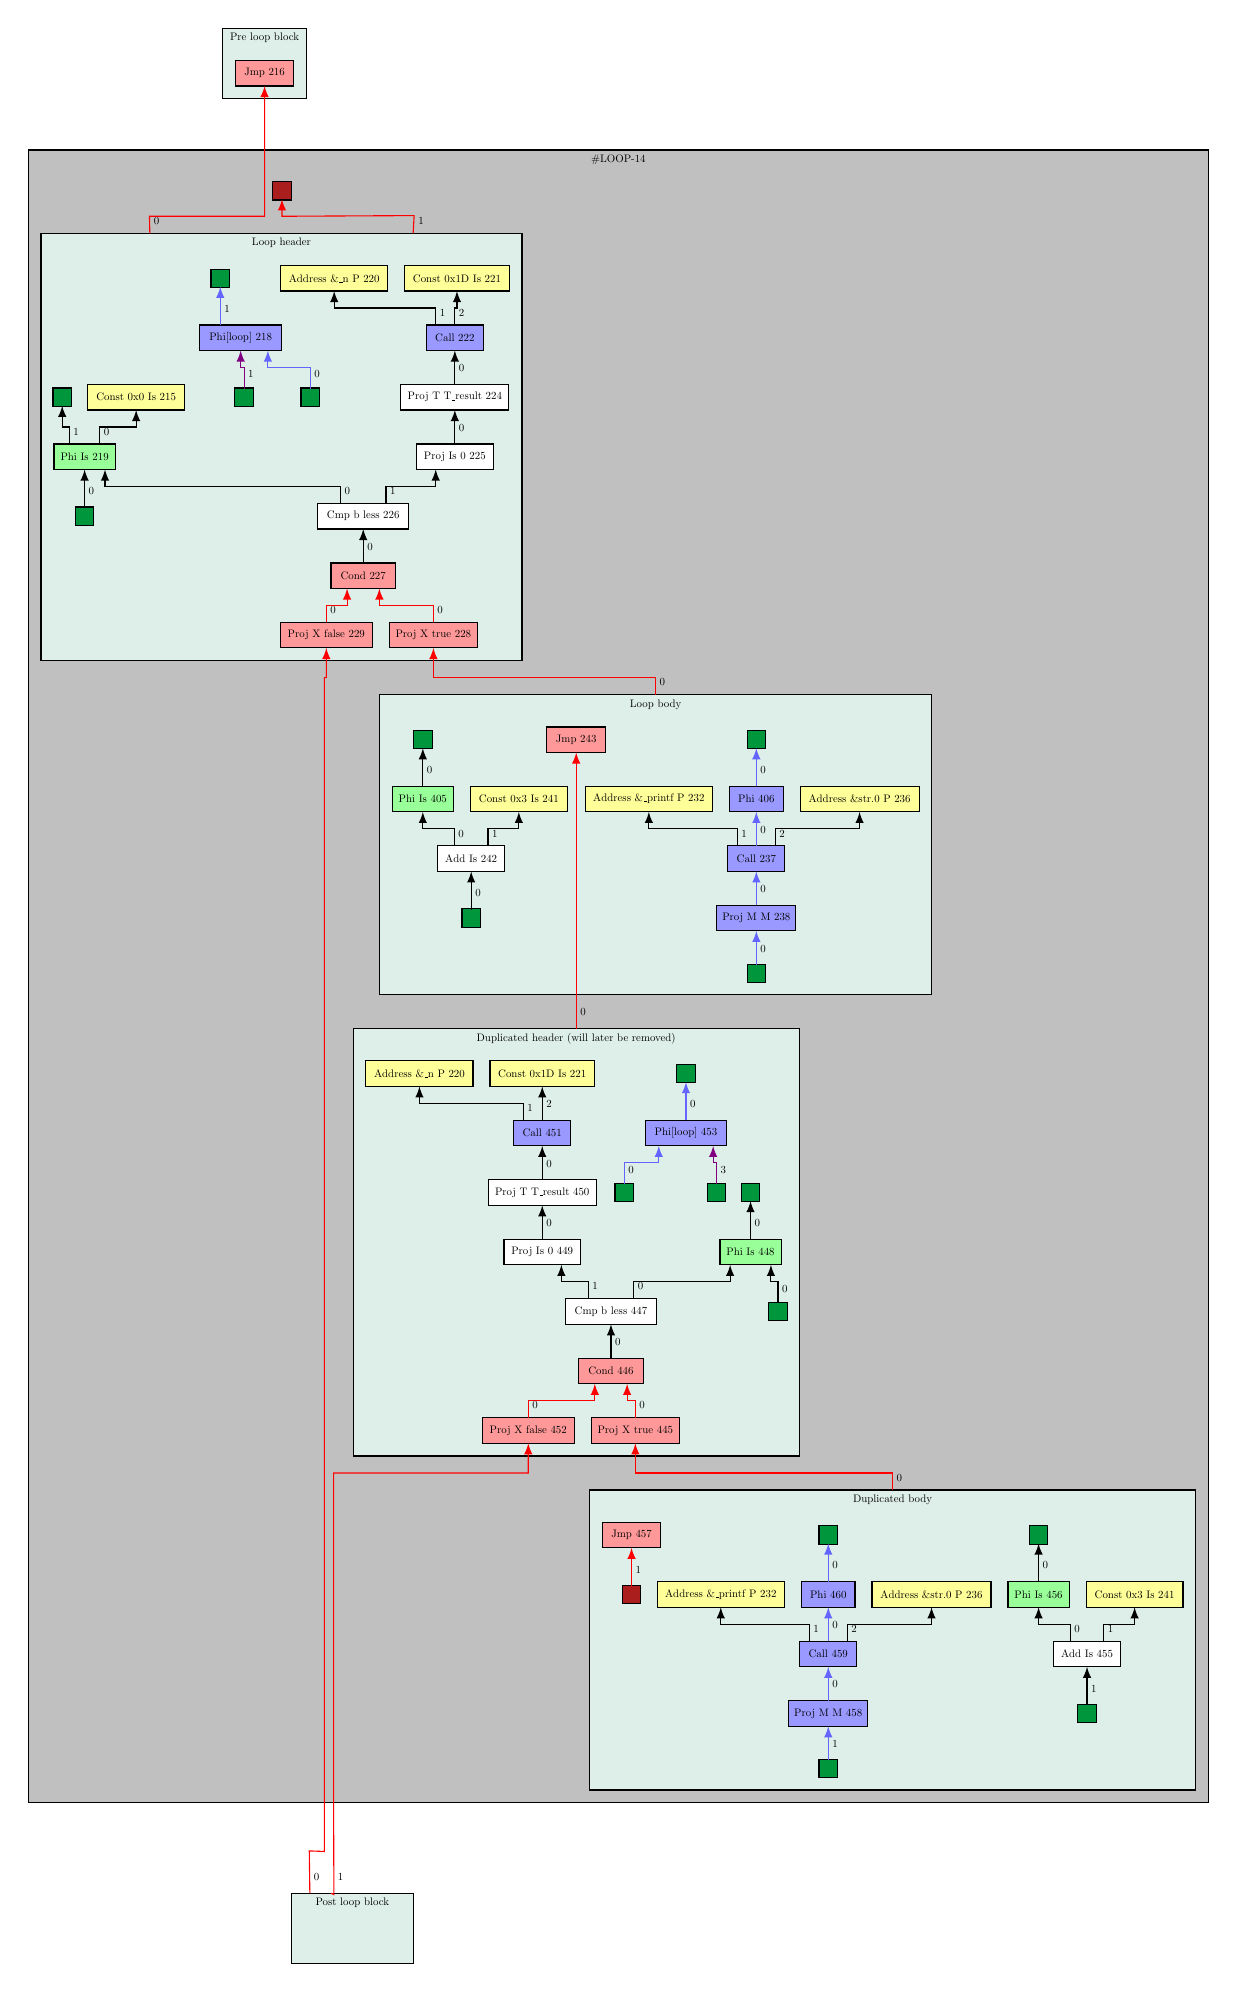
\begin{tikzpicture}
	\node[fill=color33, draw, minimum width=1.0683453237410072cm, minimum height=0.8956834532374102cm] (n101) at (11.222505742415636cm ,22.552094823164907cm) {};
	\node[fill=color34, draw, minimum width=14.989502857940924cm, minimum height=20.989208633093526cm] (n107) at (15.71598787432375cm ,10.958633093525181cm) {};
	% 1 node layouts
	\node[scale=0.3924133420536298, transform shape] at (11.222505742415636cm ,22.87667890589872cm) {Pre loop block};
	\node[fill=color33, draw, minimum width=7.699640287769787cm, minimum height=3.809352517985612cm] (n102) at (19.199048655812195cm ,2.5305755395683454cm) {};
	% 1 node layouts
	\node[scale=0.3924133420536298, transform shape] at (19.199048655812195cm ,4.311994154676259cm) {Duplicated body};
	\node[fill=color33, draw, minimum width=6.108812949640288cm, minimum height=5.428057553956835cm] (n103) at (11.437513423770554cm ,17.681654676258994cm) {};
	% 1 node layouts
	\node[scale=0.3924133420536298, transform shape] at (11.437513423770554cm ,20.27242580935252cm) {Loop header};
	\node[fill=color33, draw, minimum width=7.014388489208634cm, minimum height=3.809352517985612cm] (n104) at (16.189541668100926cm ,12.631294964028777cm) {};
	% 1 node layouts
	\node[scale=0.3924133420536298, transform shape] at (16.189541668100926cm ,14.41271357913669cm) {Loop body};
	\node[fill=color33, draw, minimum width=5.664977109221715cm, minimum height=5.428057553956835cm] (n105) at (15.18054886234553cm ,7.580935251798562cm) {};
	% 1 node layouts
	\node[scale=0.3924133420536298, transform shape] at (15.18054886234553cm ,10.171706384892087cm) {Duplicated header (will later be removed)};
	\node[fill=color33, draw, minimum width=1.5539568345323742cm, minimum height=0.8956834532374102cm] (n106) at (12.337230215827338cm ,-1.1337679856115108cm) {};
	% 1 node layouts
	\node[scale=0.3924133420536298, transform shape] at (12.337230215827338cm ,-0.8091839028776979cm) {Post loop block};
	% 1 node layouts
	\node[scale=0.3924133420536298, transform shape] at (15.71598787432375cm ,21.32997976618705cm) {\#LOOP-14};
	\node[fill=color35, draw, minimum width=0.7446043165467626cm, minimum height=0.32374100719424465cm] (n108) at (11.222505742415636cm ,22.427994103740446cm) {};
	% 1 node layouts
	\node[scale=0.3924133420536298, transform shape] at (11.222505742415636cm ,22.427994103740446cm) {Jmp  216};
	\node[fill=color36, draw, minimum width=1.0359712230215827cm, minimum height=0.32374100719424465cm] (n109) at (16.57429068706757cm ,8.967625899280575cm) {};
	% 1 node layouts
	\node[scale=0.3924133420536298, transform shape] at (16.57429068706757cm ,8.967625899280575cm) {Phi[loop]  453};
	\node[fill=color35, draw, minimum width=1.1654676258992807cm, minimum height=0.32374100719424465cm] (n110) at (14.571858541874635cm ,5.190647482014389cm) {};
	% 1 node layouts
	\node[scale=0.3924133420536298, transform shape] at (14.571858541874635cm ,5.190647482014389cm) {Proj X false 452};
	\node[fill=color35, draw, minimum width=1.1223021582733814cm, minimum height=0.32374100719424465cm] (n111) at (15.931570772090462cm ,5.190647482014389cm) {};
	% 1 node layouts
	\node[scale=0.3924133420536298, transform shape] at (15.931570772090462cm ,5.190647482014389cm) {Proj X true 445};
	\node[fill=color35, draw, minimum width=0.8201438848920863cm, minimum height=0.32374100719424465cm] (n112) at (15.62195255757117cm ,5.946043165467626cm) {};
	% 1 node layouts
	\node[scale=0.3924133420536298, transform shape] at (15.62195255757117cm ,5.946043165467626cm) {Cond  446};
	\node[fill=color37, draw, minimum width=1.154676258992806cm, minimum height=0.32374100719424465cm] (n113) at (15.62195255757117cm ,6.701438848920864cm) {};
	% 1 node layouts
	\node[scale=0.3924133420536298, transform shape] at (15.62195255757117cm ,6.701438848920864cm) {Cmp b less 447};
	\node[fill=color38, draw, minimum width=0.7769784172661871cm, minimum height=0.32374100719424465cm] (n114) at (17.394434571959657cm ,7.456834532374101cm) {};
	% 1 node layouts
	\node[scale=0.3924133420536298, transform shape] at (17.394434571959657cm ,7.456834532374101cm) {Phi Is 448};
	\node[fill=color37, draw, minimum width=0.9712230215827339cm, minimum height=0.32374100719424465cm] (n115) at (14.749139444425321cm ,7.456834532374101cm) {};
	% 1 node layouts
	\node[scale=0.3924133420536298, transform shape] at (14.749139444425321cm ,7.456834532374101cm) {Proj Is 0 449};
	\node[fill=color37, draw, minimum width=1.3705035971223023cm, minimum height=0.32374100719424465cm] (n116) at (14.749139444425321cm ,8.212230215827338cm) {};
	% 1 node layouts
	\node[scale=0.3924133420536298, transform shape] at (14.749139444425321cm ,8.212230215827338cm) {Proj T T\_result 450};
	\node[fill=color36, draw, minimum width=0.723021582733813cm, minimum height=0.32374100719424465cm] (n117) at (14.749139444425321cm ,8.967625899280575cm) {};
	% 1 node layouts
	\node[scale=0.3924133420536298, transform shape] at (14.749139444425321cm ,8.967625899280575cm) {Call  451};
	\node[fill=color39, draw, minimum width=1.3597122302158273cm, minimum height=0.32374100719424465cm] (n118) at (13.189786926439709cm ,9.723021582733814cm) {};
	% 1 node layouts
	\node[scale=0.3924133420536298, transform shape] at (13.189786926439709cm ,9.723021582733814cm) {Address \&\_n P 220};
	\node[fill=color39, draw, minimum width=1.3273381294964028cm, minimum height=0.32374100719424465cm] (n119) at (14.749139444425321cm ,9.723021582733814cm) {};
	% 1 node layouts
	\node[scale=0.3924133420536298, transform shape] at (14.749139444425321cm ,9.723021582733814cm) {Const 0x1D Is 221};
	\node[fill=color40, draw, minimum width=0.21582733812949642cm, minimum height=0.21582733812949642cm] (n120) at (15.79050635090014cm ,8.212230215827338cm) {};
	\node[fill=color40, draw, minimum width=0.21582733812949642cm, minimum height=0.21582733812949642cm] (n121) at (17.743253244294518cm ,6.701438848920864cm) {};
	\node[fill=color40, draw, minimum width=0.21582733812949642cm, minimum height=0.21582733812949642cm] (n122) at (16.57429068706757cm ,9.723021582733814cm) {};
	\node[fill=color40, draw, minimum width=0.21582733812949642cm, minimum height=0.21582733812949642cm] (n123) at (17.394434571959657cm ,8.212230215827338cm) {};
	\node[fill=color40, draw, minimum width=0.21582733812949642cm, minimum height=0.21582733812949642cm] (n124) at (16.962779895700667cm ,8.212230215827338cm) {};
	\node[fill=color36, draw, minimum width=1.0035971223021583cm, minimum height=0.32374100719424465cm] (n125) at (18.381602612646724cm ,1.5971223021582734cm) {};
	% 1 node layouts
	\node[scale=0.3924133420536298, transform shape] at (18.381602612646724cm ,1.5971223021582734cm) {Proj M M 458};
	\node[fill=color36, draw, minimum width=0.723021582733813cm, minimum height=0.32374100719424465cm] (n126) at (18.381602612646724cm ,2.352517985611511cm) {};
	% 1 node layouts
	\node[scale=0.3924133420536298, transform shape] at (18.381602612646724cm ,2.352517985611511cm) {Call  459};
	\node[fill=color39, draw, minimum width=1.6187050359712232cm, minimum height=0.32374100719424465cm] (n127) at (17.01649469897766cm ,3.1079136690647484cm) {};
	% 1 node layouts
	\node[scale=0.3924133420536298, transform shape] at (17.01649469897766cm ,3.1079136690647484cm) {Address \&\_printf P 232};
	\node[fill=color39, draw, minimum width=1.510791366906475cm, minimum height=0.32374100719424465cm] (n128) at (19.692753691783416cm ,3.1079136690647484cm) {};
	% 1 node layouts
	\node[scale=0.3924133420536298, transform shape] at (19.692753691783416cm ,3.1079136690647484cm) {Address \&str.0 P 236};
	\node[fill=color36, draw, minimum width=0.6798561151079137cm, minimum height=0.32374100719424465cm] (n129) at (18.381602612646724cm ,3.1079136690647484cm) {};
	% 1 node layouts
	\node[scale=0.3924133420536298, transform shape] at (18.381602612646724cm ,3.1079136690647484cm) {Phi  460};
	\node[fill=color35, draw, minimum width=0.7446043165467626cm, minimum height=0.32374100719424465cm] (n130) at (15.883401173797804cm ,3.863309352517986cm) {};
	% 1 node layouts
	\node[scale=0.3924133420536298, transform shape] at (15.883401173797804cm ,3.863309352517986cm) {Jmp  457};
	\node[fill=color37, draw, minimum width=0.8525179856115108cm, minimum height=0.32374100719424465cm] (n131) at (21.66795924162925cm ,2.352517985611511cm) {};
	% 1 node layouts
	\node[scale=0.3924133420536298, transform shape] at (21.66795924162925cm ,2.352517985611511cm) {Add Is 455};
	\node[fill=color39, draw, minimum width=1.2302158273381296cm, minimum height=0.32374100719424465cm] (n132) at (22.2718903824309cm ,3.1079136690647484cm) {};
	% 1 node layouts
	\node[scale=0.3924133420536298, transform shape] at (22.2718903824309cm ,3.1079136690647484cm) {Const 0x3 Is 241};
	\node[fill=color38, draw, minimum width=0.7769784172661871cm, minimum height=0.32374100719424465cm] (n133) at (21.052465921999243cm ,3.1079136690647484cm) {};
	% 1 node layouts
	\node[scale=0.3924133420536298, transform shape] at (21.052465921999243cm ,3.1079136690647484cm) {Phi Is 456};
	\node[fill=color40, draw, minimum width=0.21582733812949642cm, minimum height=0.21582733812949642cm] (n134) at (18.381602612646724cm ,3.863309352517986cm) {};
	\node[fill=color40, draw, minimum width=0.21582733812949642cm, minimum height=0.21582733812949642cm] (n135) at (21.052465921999243cm ,3.863309352517986cm) {};
	\node[fill=color40, draw, minimum width=0.21582733812949642cm, minimum height=0.21582733812949642cm] (n136) at (18.381602612646724cm ,0.8956834532374102cm) {};
	\node[fill=color40, draw, minimum width=0.21582733812949642cm, minimum height=0.21582733812949642cm] (n137) at (21.66795924162925cm ,1.5971223021582734cm) {};
	\node[fill=color36, draw, minimum width=1.0359712230215827cm, minimum height=0.32374100719424465cm] (n138) at (10.919078171971991cm ,19.06834532374101cm) {};
	% 1 node layouts
	\node[scale=0.3924133420536298, transform shape] at (10.919078171971991cm ,19.06834532374101cm) {Phi[loop]  218};
	\node[fill=color35, draw, minimum width=1.1654676258992807cm, minimum height=0.32374100719424465cm] (n139) at (12.006851703147051cm ,15.29136690647482cm) {};
	% 1 node layouts
	\node[scale=0.3924133420536298, transform shape] at (12.006851703147051cm ,15.29136690647482cm) {Proj X false 229};
	\node[fill=color35, draw, minimum width=1.1223021582733814cm, minimum height=0.32374100719424465cm] (n140) at (13.366563933362878cm ,15.29136690647482cm) {};
	% 1 node layouts
	\node[scale=0.3924133420536298, transform shape] at (13.366563933362878cm ,15.29136690647482cm) {Proj X true 228};
	\node[fill=color35, draw, minimum width=0.8201438848920863cm, minimum height=0.32374100719424465cm] (n141) at (12.475732848230985cm ,16.046762589928058cm) {};
	% 1 node layouts
	\node[scale=0.3924133420536298, transform shape] at (12.475732848230985cm ,16.046762589928058cm) {Cond  227};
	\node[fill=color37, draw, minimum width=1.154676258992806cm, minimum height=0.32374100719424465cm] (n142) at (12.475732848230985cm ,16.802158273381295cm) {};
	% 1 node layouts
	\node[scale=0.3924133420536298, transform shape] at (12.475732848230985cm ,16.802158273381295cm) {Cmp b less 226};
	\node[fill=color37, draw, minimum width=0.9712230215827339cm, minimum height=0.32374100719424465cm] (n143) at (13.63915835782331cm ,17.557553956834532cm) {};
	% 1 node layouts
	\node[scale=0.3924133420536298, transform shape] at (13.63915835782331cm ,17.557553956834532cm) {Proj Is 0 225};
	\node[fill=color37, draw, minimum width=1.3705035971223023cm, minimum height=0.32374100719424465cm] (n144) at (13.63915835782331cm ,18.31294964028777cm) {};
	% 1 node layouts
	\node[scale=0.3924133420536298, transform shape] at (13.63915835782331cm ,18.31294964028777cm) {Proj T T\_result 224};
	\node[fill=color36, draw, minimum width=0.723021582733813cm, minimum height=0.32374100719424465cm] (n145) at (13.63915835782331cm ,19.06834532374101cm) {};
	% 1 node layouts
	\node[scale=0.3924133420536298, transform shape] at (13.63915835782331cm ,19.06834532374101cm) {Call  222};
	\node[fill=color39, draw, minimum width=1.3597122302158273cm, minimum height=0.32374100719424465cm] (n146) at (12.10702781225976cm ,19.823741007194247cm) {};
	% 1 node layouts
	\node[scale=0.3924133420536298, transform shape] at (12.10702781225976cm ,19.823741007194247cm) {Address \&\_n P 220};
	\node[fill=color39, draw, minimum width=1.3273381294964028cm, minimum height=0.32374100719424465cm] (n147) at (13.666380330245373cm ,19.823741007194247cm) {};
	% 1 node layouts
	\node[scale=0.3924133420536298, transform shape] at (13.666380330245373cm ,19.823741007194247cm) {Const 0x1D Is 221};
	\node[fill=color38, draw, minimum width=0.7769784172661871cm, minimum height=0.32374100719424465cm] (n148) at (8.937157458542735cm ,17.557553956834532cm) {};
	% 1 node layouts
	\node[scale=0.3924133420536298, transform shape] at (8.937157458542735cm ,17.557553956834532cm) {Phi Is 219};
	\node[fill=color39, draw, minimum width=1.2302158273381296cm, minimum height=0.32374100719424465cm] (n149) at (9.591740042475589cm ,18.31294964028777cm) {};
	% 1 node layouts
	\node[scale=0.3924133420536298, transform shape] at (9.591740042475589cm ,18.31294964028777cm) {Const 0x0 Is 215};
	\node[fill=color40, draw, minimum width=0.21582733812949642cm, minimum height=0.21582733812949642cm] (n150) at (10.660085366216595cm ,19.823741007194247cm) {};
	\node[fill=color40, draw, minimum width=0.21582733812949642cm, minimum height=0.21582733812949642cm] (n151) at (8.65289112161228cm ,18.31294964028777cm) {};
	\node[fill=color40, draw, minimum width=0.21582733812949642cm, minimum height=0.21582733812949642cm] (n152) at (11.802902362619474cm ,18.31294964028777cm) {};
	\node[fill=color40, draw, minimum width=0.21582733812949642cm, minimum height=0.21582733812949642cm] (n153) at (8.937157458542735cm ,16.802158273381295cm) {};
	\node[fill=color40, draw, minimum width=0.21582733812949642cm, minimum height=0.21582733812949642cm] (n154) at (10.96224363959789cm ,18.31294964028777cm) {};
	\node[fill=color36, draw, minimum width=1.0035971223021583cm, minimum height=0.32374100719424465cm] (n155) at (17.468318646518192cm ,11.697841726618705cm) {};
	% 1 node layouts
	\node[scale=0.3924133420536298, transform shape] at (17.468318646518192cm ,11.697841726618705cm) {Proj M M 238};
	\node[fill=color36, draw, minimum width=0.723021582733813cm, minimum height=0.32374100719424465cm] (n156) at (17.468318646518192cm ,12.453237410071942cm) {};
	% 1 node layouts
	\node[scale=0.3924133420536298, transform shape] at (17.468318646518192cm ,12.453237410071942cm) {Call  237};
	\node[fill=color39, draw, minimum width=1.6187050359712232cm, minimum height=0.32374100719424465cm] (n157) at (16.103210732849128cm ,13.208633093525181cm) {};
	% 1 node layouts
	\node[scale=0.3924133420536298, transform shape] at (16.103210732849128cm ,13.208633093525181cm) {Address \&\_printf P 232};
	\node[fill=color39, draw, minimum width=1.510791366906475cm, minimum height=0.32374100719424465cm] (n158) at (18.77946972565488cm ,13.208633093525181cm) {};
	% 1 node layouts
	\node[scale=0.3924133420536298, transform shape] at (18.77946972565488cm ,13.208633093525181cm) {Address \&str.0 P 236};
	\node[fill=color36, draw, minimum width=0.6798561151079137cm, minimum height=0.32374100719424465cm] (n159) at (17.468318646518192cm ,13.208633093525181cm) {};
	% 1 node layouts
	\node[scale=0.3924133420536298, transform shape] at (17.468318646518192cm ,13.208633093525181cm) {Phi  406};
	\node[fill=color35, draw, minimum width=0.7446043165467626cm, minimum height=0.32374100719424465cm] (n160) at (15.18054886234553cm ,13.964028776978418cm) {};
	% 1 node layouts
	\node[scale=0.3924133420536298, transform shape] at (15.18054886234553cm ,13.964028776978418cm) {Jmp  243};
	\node[fill=color37, draw, minimum width=0.8525179856115108cm, minimum height=0.32374100719424465cm] (n161) at (13.84691576882035cm ,12.453237410071942cm) {};
	% 1 node layouts
	\node[scale=0.3924133420536298, transform shape] at (13.84691576882035cm ,12.453237410071942cm) {Add Is 242};
	\node[fill=color39, draw, minimum width=1.2302158273381296cm, minimum height=0.32374100719424465cm] (n162) at (14.452131596158479cm ,13.208633093525181cm) {};
	% 1 node layouts
	\node[scale=0.3924133420536298, transform shape] at (14.452131596158479cm ,13.208633093525181cm) {Const 0x3 Is 241};
	\node[fill=color38, draw, minimum width=0.7769784172661871cm, minimum height=0.32374100719424465cm] (n163) at (13.232707135726825cm ,13.208633093525181cm) {};
	% 1 node layouts
	\node[scale=0.3924133420536298, transform shape] at (13.232707135726825cm ,13.208633093525181cm) {Phi Is 405};
	\node[fill=color40, draw, minimum width=0.21582733812949642cm, minimum height=0.21582733812949642cm] (n164) at (17.468318646518192cm ,13.964028776978418cm) {};
	\node[fill=color40, draw, minimum width=0.21582733812949642cm, minimum height=0.21582733812949642cm] (n165) at (13.232707135726825cm ,13.964028776978418cm) {};
	\node[fill=color40, draw, minimum width=0.21582733812949642cm, minimum height=0.21582733812949642cm] (n166) at (17.468318646518192cm ,10.996402877697843cm) {};
	\node[fill=color40, draw, minimum width=0.21582733812949642cm, minimum height=0.21582733812949642cm] (n167) at (13.84691576882035cm ,11.697841726618705cm) {};
	\node[fill=color41, draw, minimum width=0.21582733812949642cm, minimum height=0.21582733812949642cm] (n168) at (11.44372876399837cm ,20.93525179856115cm) {};
	\node[fill=color41, draw, minimum width=0.21582733812949642cm, minimum height=0.21582733812949642cm] (n169) at (15.883401173797804cm ,3.1079136690647484cm) {};
	\draw[color=color42, -latex] (19.199048655812195cm ,4.4352517985611515cm) -- (19.19904865581219cm ,4.651079136690647cm) -- (15.931570772090462cm ,4.651079136690647cm) -- (15.931570772090462cm ,5.028776978417266cm);
	\node[] at (19.285379591063993cm ,4.592401079136691cm) {
		\scalebox{0.3924133420536298}{0}
	};
	\draw[color=color42, -latex] (9.7655494324636cm ,20.39568345323741cm) -- (9.760920011000769cm ,20.611510791366907cm) -- (11.222505742415636cm ,20.611510791366907cm) -- (11.222505742415636cm ,22.266123600143324cm);
	\node[] at (9.850608180996998cm ,20.552832733812952cm) {
		\scalebox{0.3924133420536298}{0}
	};
	\draw[color=color42, -latex] (16.189541668100926cm ,14.535971223021583cm) -- (16.189541668100926cm ,14.75179856115108cm) -- (13.366563933362878cm ,14.75179856115108cm) -- (13.366563933362878cm ,15.129496402877699cm);
	\node[] at (16.275872603352724cm ,14.693120503597124cm) {
		\scalebox{0.3924133420536298}{0}
	};
	\draw[color=color42, -latex] (15.18054886234553cm ,10.29496402877698cm) -- (15.18054886234553cm ,13.802158273381295cm);
	\node[] at (15.266879797597328cm ,10.502065535071942cm) {
		\scalebox{0.3924133420536298}{0}
	};
	\draw[color=color42, -latex] (11.797661870503598cm ,-0.6858714590827368cm) -- (11.790546954690896cm ,-0.14814226901732497cm) -- (11.981892086330935cm ,-0.15513669064747931cm) -- (11.981545385701008cm ,0.24820143884892087cm) -- (11.981545385701008cm ,14.75179856115108cm) -- (12.006851703147051cm ,14.75179856115108cm) -- (12.006851703147051cm ,15.129496402877699cm);
	\node[] at (11.88254783262315cm ,-0.47882475269784175cm) {
		\scalebox{0.3924133420536298}{0}
	};
	\draw[color=color42, -latex] (12.067446043165468cm ,-0.6858714590827368cm) -- (12.103153327338127cm ,-0.7027877697841727cm) -- (12.100250421672232cm ,0.14028776978417268cm) -- (12.100250421672232cm ,4.651079136690647cm) -- (14.571858541874635cm ,4.651079136690647cm) -- (14.571858541874635cm ,5.028776978417266cm);
	\node[] at (12.189049987902306cm ,-0.47882475269784175cm) {
		\scalebox{0.3924133420536298}{1}
	};
	\draw[color=color43, -latex] (16.57429068706757cm ,9.129496402877699cm) -- (16.57429068706757cm ,9.615107913669066cm);
	\node[] at (16.660621622319372cm ,9.336597909172662cm) {
		\scalebox{0.3924133420536298}{0}
	};
	\draw[color=color42, -latex] (14.571858541874635cm ,5.352517985611511cm) -- (14.571858541874635cm ,5.568345323741007cm) -- (15.416916586348147cm ,5.568345323741007cm) -- (15.416916586348147cm ,5.784172661870504cm);
	\node[] at (14.658189477126433cm ,5.5096672661870505cm) {
		\scalebox{0.3924133420536298}{0}
	};
	\draw[color=color42, -latex] (15.931570772090462cm ,5.352517985611511cm) -- (15.931570772090462cm ,5.568345323741007cm) -- (15.82698852879419cm ,5.568345323741007cm) -- (15.82698852879419cm ,5.784172661870504cm);
	\node[] at (16.01790170734226cm ,5.5096672661870505cm) {
		\scalebox{0.3924133420536298}{0}
	};
	\draw[color=color44, -latex] (15.62195255757117cm ,6.107913669064748cm) -- (15.62195255757117cm ,6.539568345323741cm);
	\node[] at (15.708283492822968cm ,6.315015175359712cm) {
		\scalebox{0.3924133420536298}{0}
	};
	\draw[color=color44, -latex] (15.91062162231937cm ,6.863309352517986cm) -- (15.91062162231937cm ,7.079136690647482cm) -- (17.135441766204263cm ,7.079136690647482cm) -- (17.135441766204263cm ,7.294964028776978cm);
	\node[] at (15.99695255757117cm ,7.020458633093526cm) {
		\scalebox{0.3924133420536298}{0}
	};
	\draw[color=color44, -latex] (15.333283492822968cm ,6.863309352517986cm) -- (15.333283492822968cm ,7.079136690647482cm) -- (14.991945199821004cm ,7.079136690647482cm) -- (14.991945199821004cm ,7.294964028776978cm);
	\node[] at (15.419614428074766cm ,7.020458633093526cm) {
		\scalebox{0.3924133420536298}{1}
	};
	\draw[color=color44, -latex] (17.394434571959657cm ,7.618705035971224cm) -- (17.394434571959657cm ,8.10431654676259cm);
	\node[] at (17.48076550721146cm ,7.8258065422661875cm) {
		\scalebox{0.3924133420536298}{0}
	};
	\draw[color=color44, -latex] (14.749139444425321cm ,7.618705035971224cm) -- (14.749139444425321cm ,8.050359712230216cm);
	\node[] at (14.835470379677119cm ,7.8258065422661875cm) {
		\scalebox{0.3924133420536298}{0}
	};
	\draw[color=color44, -latex] (14.749139444425321cm ,8.374100719424462cm) -- (14.749139444425321cm ,8.805755395683454cm);
	\node[] at (14.835470379677119cm ,8.581202225719425cm) {
		\scalebox{0.3924133420536298}{0}
	};
	\draw[color=color44, -latex] (14.508132250180717cm ,9.129496402877699cm) -- (14.508132250180717cm ,9.345323741007194cm) -- (13.189786926439709cm ,9.345323741007194cm) -- (13.189786926439709cm ,9.56115107913669cm);
	\node[] at (14.594463185432515cm ,9.286645683453237cm) {
		\scalebox{0.3924133420536298}{1}
	};
	\draw[color=color44, -latex] (14.749139444425321cm ,9.129496402877699cm) -- (14.749139444425321cm ,9.56115107913669cm);
	\node[] at (14.835470379677119cm ,9.336597909172662cm) {
		\scalebox{0.3924133420536298}{2}
	};
	\draw[color=color43, -latex] (15.79050635090014cm ,8.320143884892087cm) -- (15.79050635090014cm ,8.589928057553957cm) -- (16.22896694606038cm ,8.589928057553957cm) -- (16.22896694606038cm ,8.805755395683454cm);
	\node[] at (15.87683728615194cm ,8.504271582733814cm) {
		\scalebox{0.3924133420536298}{0}
	};
	\draw[color=color44, -latex] (17.743253244294518cm ,6.809352517985612cm) -- (17.743253244294518cm ,7.079136690647482cm) -- (17.653427377715055cm ,7.079136690647482cm) -- (17.653427377715055cm ,7.294964028776978cm);
	\node[] at (17.829584179546316cm ,6.993480215827338cm) {
		\scalebox{0.3924133420536298}{0}
	};
	\draw[color=color45, -latex] (16.962779895700667cm ,8.320143884892087cm) -- (16.962779895700667cm ,8.589928057553957cm) -- (16.919614428074766cm ,8.589928057553957cm) -- (16.919614428074766cm ,8.805755395683454cm);
	\node[] at (17.049110830952465cm ,8.504271582733814cm) {
		\scalebox{0.3924133420536298}{3}
	};
	\draw[color=color43, -latex] (18.381602612646724cm ,1.7589928057553958cm) -- (18.381602612646724cm ,2.1906474820143886cm);
	\node[] at (18.467933547898525cm ,1.9660943120503598cm) {
		\scalebox{0.3924133420536298}{0}
	};
	\draw[color=color43, -latex] (18.381602612646724cm ,2.514388489208633cm) -- (18.381602612646724cm ,2.9460431654676262cm);
	\node[] at (18.467933547898525cm ,2.7214899955035974cm) {
		\scalebox{0.3924133420536298}{0}
	};
	\draw[color=color44, -latex] (18.14059541840212cm ,2.514388489208633cm) -- (18.14059541840212cm ,2.73021582733813cm) -- (17.01649469897766cm ,2.73021582733813cm) -- (17.01649469897766cm ,2.9460431654676262cm);
	\node[] at (18.22692635365392cm ,2.6715377697841727cm) {
		\scalebox{0.3924133420536298}{1}
	};
	\draw[color=color44, -latex] (18.62260980689133cm ,2.514388489208633cm) -- (18.62260980689133cm ,2.73021582733813cm) -- (19.692753691783416cm ,2.73021582733813cm) -- (19.692753691783416cm ,2.9460431654676262cm);
	\node[] at (18.708940742143128cm ,2.6715377697841727cm) {
		\scalebox{0.3924133420536298}{2}
	};
	\draw[color=color43, -latex] (18.381602612646724cm ,3.2697841726618706cm) -- (18.381602612646724cm ,3.7553956834532376cm);
	\node[] at (18.467933547898525cm ,3.4768856789568345cm) {
		\scalebox{0.3924133420536298}{0}
	};
	\draw[color=color44, -latex] (21.454829745226377cm ,2.514388489208633cm) -- (21.454829745226377cm ,2.73021582733813cm) -- (21.052465921999243cm ,2.73021582733813cm) -- (21.052465921999243cm ,2.9460431654676262cm);
	\node[] at (21.541160680478175cm ,2.6715377697841727cm) {
		\scalebox{0.3924133420536298}{0}
	};
	\draw[color=color44, -latex] (21.88108873803213cm ,2.514388489208633cm) -- (21.88108873803213cm ,2.73021582733813cm) -- (22.2718903824309cm ,2.73021582733813cm) -- (22.2718903824309cm ,2.9460431654676262cm);
	\node[] at (21.967419673283928cm ,2.6715377697841727cm) {
		\scalebox{0.3924133420536298}{1}
	};
	\draw[color=color44, -latex] (21.052465921999243cm ,3.2697841726618706cm) -- (21.052465921999243cm ,3.7553956834532376cm);
	\node[] at (21.13879685725104cm ,3.4768856789568345cm) {
		\scalebox{0.3924133420536298}{0}
	};
	\draw[color=color43, -latex] (18.381602612646724cm ,1.0035971223021583cm) -- (18.381602612646724cm ,1.4352517985611513cm);
	\node[] at (18.467933547898525cm ,1.2106986285971224cm) {
		\scalebox{0.3924133420536298}{1}
	};
	\draw[color=color44, -latex] (21.66795924162925cm ,1.7050359712230216cm) -- (21.66795924162925cm ,2.1906474820143886cm);
	\node[] at (21.754290176881053cm ,1.9121374775179858cm) {
		\scalebox{0.3924133420536298}{1}
	};
	\draw[color=color43, -latex] (10.660085366216595cm ,19.23021582733813cm) -- (10.660085366216595cm ,19.715827338129497cm);
	\node[] at (10.746416301468393cm ,19.437317333633093cm) {
		\scalebox{0.3924133420536298}{1}
	};
	\draw[color=color42, -latex] (12.006851703147051cm ,15.453237410071944cm) -- (12.006851703147051cm ,15.66906474820144cm) -- (12.270696877007962cm ,15.66906474820144cm) -- (12.270696877007962cm ,15.884892086330936cm);
	\node[] at (12.093182638398849cm ,15.610386690647482cm) {
		\scalebox{0.3924133420536298}{0}
	};
	\draw[color=color42, -latex] (13.366563933362878cm ,15.453237410071944cm) -- (13.366563933362878cm ,15.66906474820144cm) -- (12.680768819454006cm ,15.66906474820144cm) -- (12.680768819454006cm ,15.884892086330936cm);
	\node[] at (13.452894868614676cm ,15.610386690647482cm) {
		\scalebox{0.3924133420536298}{0}
	};
	\draw[color=color44, -latex] (12.475732848230985cm ,16.20863309352518cm) -- (12.475732848230985cm ,16.640287769784173cm);
	\node[] at (12.562063783482783cm ,16.415734599820144cm) {
		\scalebox{0.3924133420536298}{0}
	};
	\draw[color=color44, -latex] (12.187063783482783cm ,16.964028776978417cm) -- (12.187063783482783cm ,17.179856115107913cm) -- (9.196150264298131cm ,17.179856115107913cm) -- (9.196150264298131cm ,17.39568345323741cm);
	\node[] at (12.27339471873458cm ,17.12117805755396cm) {
		\scalebox{0.3924133420536298}{0}
	};
	\draw[color=color44, -latex] (12.764401912979185cm ,16.964028776978417cm) -- (12.764401912979185cm ,17.179856115107913cm) -- (13.396352602427626cm ,17.179856115107913cm) -- (13.396352602427626cm ,17.39568345323741cm);
	\node[] at (12.850732848230985cm ,17.12117805755396cm) {
		\scalebox{0.3924133420536298}{1}
	};
	\draw[color=color44, -latex] (13.63915835782331cm ,17.719424460431657cm) -- (13.63915835782331cm ,18.151079136690647cm);
	\node[] at (13.725489293075109cm ,17.92652596672662cm) {
		\scalebox{0.3924133420536298}{0}
	};
	\draw[color=color44, -latex] (13.63915835782331cm ,18.474820143884894cm) -- (13.63915835782331cm ,18.906474820143885cm);
	\node[] at (13.725489293075109cm ,18.681921650179856cm) {
		\scalebox{0.3924133420536298}{0}
	};
	\draw[color=color44, -latex] (13.398151163578707cm ,19.23021582733813cm) -- (13.398151163578707cm ,19.44604316546763cm) -- (12.10702781225976cm ,19.44604316546763cm) -- (12.10702781225976cm ,19.66187050359712cm);
	\node[] at (13.484482098830506cm ,19.38736510791367cm) {
		\scalebox{0.3924133420536298}{1}
	};
	\draw[color=color44, -latex] (13.63915835782331cm ,19.23021582733813cm) -- (13.63915835782331cm ,19.44604316546763cm) -- (13.666380330245373cm ,19.44604316546763cm) -- (13.666380330245373cm ,19.66187050359712cm);
	\node[] at (13.725489293075109cm ,19.38736510791367cm) {
		\scalebox{0.3924133420536298}{2}
	};
	\draw[color=color44, -latex] (9.131402062859282cm ,17.719424460431657cm) -- (9.131402062859282cm ,17.93525179856115cm) -- (9.591740042475589cm ,17.93525179856115cm) -- (9.591740042475589cm ,18.151079136690647cm);
	\node[] at (9.21773299811108cm ,17.876573741007196cm) {
		\scalebox{0.3924133420536298}{0}
	};
	\draw[color=color44, -latex] (8.742912854226187cm ,17.719424460431657cm) -- (8.742912854226187cm ,17.93525179856115cm) -- (8.65289112161228cm ,17.93525179856115cm) -- (8.65289112161228cm ,18.205035971223023cm);
	\node[] at (8.829243789477987cm ,17.876573741007196cm) {
		\scalebox{0.3924133420536298}{1}
	};
	\draw[color=color43, -latex] (11.802902362619474cm ,18.42086330935252cm) -- (11.802902362619474cm ,18.690647482014388cm) -- (11.264401912979185cm ,18.690647482014388cm) -- (11.264401912979185cm ,18.906474820143885cm);
	\node[] at (11.889233297871273cm ,18.604991007194247cm) {
		\scalebox{0.3924133420536298}{0}
	};
	\draw[color=color44, -latex] (8.937157458542735cm ,16.910071942446045cm) -- (8.937157458542735cm ,17.39568345323741cm);
	\node[] at (9.023488393794533cm ,17.117173448741006cm) {
		\scalebox{0.3924133420536298}{0}
	};
	\draw[color=color45, -latex] (10.96224363959789cm ,18.42086330935252cm) -- (10.96224363959789cm ,18.690647482014388cm) -- (10.919078171971991cm ,18.690647482014388cm) -- (10.919078171971991cm ,18.906474820143885cm);
	\node[] at (11.048574574849688cm ,18.604991007194247cm) {
		\scalebox{0.3924133420536298}{1}
	};
	\draw[color=color43, -latex] (17.468318646518192cm ,11.859712230215829cm) -- (17.468318646518192cm ,12.29136690647482cm);
	\node[] at (17.55464958176999cm ,12.066813736510792cm) {
		\scalebox{0.3924133420536298}{0}
	};
	\draw[color=color43, -latex] (17.468318646518192cm ,12.615107913669066cm) -- (17.468318646518192cm ,13.046762589928058cm);
	\node[] at (17.55464958176999cm ,12.822209419964029cm) {
		\scalebox{0.3924133420536298}{0}
	};
	\draw[color=color44, -latex] (17.22731145227359cm ,12.615107913669066cm) -- (17.22731145227359cm ,12.830935251798563cm) -- (16.103210732849128cm ,12.830935251798563cm) -- (16.103210732849128cm ,13.046762589928058cm);
	\node[] at (17.313642387525388cm ,12.772257194244604cm) {
		\scalebox{0.3924133420536298}{1}
	};
	\draw[color=color44, -latex] (17.709325840762794cm ,12.615107913669066cm) -- (17.709325840762794cm ,12.830935251798563cm) -- (18.77946972565488cm ,12.830935251798563cm) -- (18.77946972565488cm ,13.046762589928058cm);
	\node[] at (17.795656776014592cm ,12.772257194244604cm) {
		\scalebox{0.3924133420536298}{2}
	};
	\draw[color=color43, -latex] (17.468318646518192cm ,13.370503597122303cm) -- (17.468318646518192cm ,13.85611510791367cm);
	\node[] at (17.55464958176999cm ,13.577605103417266cm) {
		\scalebox{0.3924133420536298}{0}
	};
	\draw[color=color44, -latex] (13.633786272417472cm ,12.615107913669066cm) -- (13.633786272417472cm ,12.830935251798563cm) -- (13.232707135726825cm ,12.830935251798563cm) -- (13.232707135726825cm ,13.046762589928058cm);
	\node[] at (13.720117207669272cm ,12.772257194244604cm) {
		\scalebox{0.3924133420536298}{0}
	};
	\draw[color=color44, -latex] (14.060045265223229cm ,12.615107913669066cm) -- (14.060045265223229cm ,12.830935251798563cm) -- (14.452131596158479cm ,12.830935251798563cm) -- (14.452131596158479cm ,13.046762589928058cm);
	\node[] at (14.146376200475027cm ,12.772257194244604cm) {
		\scalebox{0.3924133420536298}{1}
	};
	\draw[color=color44, -latex] (13.232707135726825cm ,13.370503597122303cm) -- (13.232707135726825cm ,13.85611510791367cm);
	\node[] at (13.319038070978623cm ,13.577605103417266cm) {
		\scalebox{0.3924133420536298}{0}
	};
	\draw[color=color43, -latex] (17.468318646518192cm ,11.10431654676259cm) -- (17.468318646518192cm ,11.535971223021583cm);
	\node[] at (17.55464958176999cm ,11.311418053057555cm) {
		\scalebox{0.3924133420536298}{0}
	};
	\draw[color=color44, -latex] (13.84691576882035cm ,11.805755395683454cm) -- (13.84691576882035cm ,12.29136690647482cm);
	\node[] at (13.933246704072149cm ,12.012856901978418cm) {
		\scalebox{0.3924133420536298}{0}
	};
	\draw[color=color42, -latex] (13.109477415077507cm ,20.39568345323741cm) -- (13.122114180665038cm ,20.620143884892087cm) -- (11.44372876399837cm ,20.611510791366907cm) -- (11.44372876399837cm ,20.827338129496404cm);
	\node[] at (13.210406795310364cm ,20.55714928057554cm) {
		\scalebox{0.3924133420536298}{1}
	};
	\draw[color=color42, -latex] (15.883401173797804cm ,3.2158273381294964cm) -- (15.883401173797804cm ,3.7014388489208634cm);
	\node[] at (15.969732109049604cm ,3.4229288444244608cm) {
		\scalebox{0.3924133420536298}{1}
	};
\end{tikzpicture}

    \end{adjustbox}
    \caption{Firm graph of the loop shown in \cref{fig:impl:unroll:unroll-factor-2-before} unrolled with a factor of two}
    \label{fig:impl:unroll:unroll-factor-2-after}
\end{figure}

\section{Fixup strategies}\label{sec:impl:fixup}

In \cref{sec:impl:unroll} the unrolling process is discussed.
That process is done without considering the fixup code needed.
In \cref{sec:impl:fixup:duff} a generalized version of duff's device will be used to create the needed fixup, whereas in \cref{sec:impl:fixup:loop} a copy of the original loop.
Later we will evaluate, which approach yields faster binary runtimes.

\subsection{Generalized duff's device}\label{sec:impl:fixup:duff}

In \cref{sec:basics:duffs}, duff's device is described and shown.
The problem with this initial approach is that it assumes $c = 1$, even though \hyperref[sec:impl::def-c]{$c$ is defined} as any non-zero integer.
Henceforth, a need for generalization arises.

Let $M \in \mathbb{Z}$ be the number of times a loop runs before the transformation; $\Mloop \in \mathbb{N}_0$, $\Mfixup \in \mathbb{N}_0$ the number of times it will run in the unrolled loop, or the fixup code respectively, after the transformation.
Further, the unroll-factor will be again denoted by $f \in \mathbb{N}, f > 1$.

\begin{equation}\label{eqn:impl:fixup:duff:conserve-semantics-identity}
    \begin{aligned}
        M = \Mloop + \Mfixup
    \end{aligned}
\end{equation}

\begin{equation}\label{eqn:impl:fixup:duff:loop-iterations}
    \begin{aligned}
        \Mloop &\overset{\text{integer divison}}{=} \frac{M}{f} \cdot f\\
        &\overset{\text{integer divison}}{\in} \medspace \rbrack M-f,f \rbrack \andinN
    \end{aligned}
\end{equation}

\begin{equation}\label{eqn:impl:fixup:duff:fixup-interval}
    \begin{aligned}
        \Mfixup \in \lbrack0, f\lbrack \medspace \andinN
    \end{aligned}
\end{equation}

\begin{equation}\label{eqn:impl:fixup:duff:total-iteration-based-on-bounds}
    \begin{aligned}
        M &= \ceil{\frac{N - I}{c}} \\
        & \overset{\text{integer divison}}{=}
        \begin{cases}
              \frac{N - I + (c - 1)}{c} &, \medspace c > 0\\
              \frac{N - I + (c + 1)}{c} &, \medspace c < 0
        \end{cases}
    \end{aligned}
\end{equation}

\begin{equation}\label{eqn:impl:fixup:duff:i-after-loop}
    \begin{aligned}
        \ipl = c \cdot \Mloop + I
    \end{aligned}
\end{equation}

\begin{equation}\label{eqn:impl:fixup:duff:fixup-i}
    \begin{aligned}
        \Mfixup & \overset{\ref{eqn:impl:fixup:duff:conserve-semantics-identity}}{=} M - \Mloop \\
        & \overset{\ref{eqn:impl:fixup:duff:total-iteration-based-on-bounds}}{=}
            \frac{N - I + (c \mp 1)}{c} - \Mloop \\
        & \overset{\ref{eqn:impl:fixup:duff:i-after-loop}}{=}
        \frac{N - I + (c \mp 1)}{c} - \frac{\ipl + I}{c} \\
        &= \frac{N - I + I - \ipl + (c \mp 1)}{c}\\
        &= \frac{N - \ipl + (c \mp 1)}{c}
    \end{aligned}
\end{equation}

\begin{equation}\label{eqn:impl:fixup:duff:fixup-i-mult}
    \begin{aligned}
        \ref{eqn:impl:fixup:duff:fixup-i} &\overset{integer division}{\Longleftrightarrow} \Mfixup \cdot c = N - \ipl + (c \mp 1) \overset{\ref{eqn:impl:fixup:duff:fixup-interval}}{\in} \cinterval
    \end{aligned}
\end{equation}

The main identity that is to be conserved, to retain the original semantics, is shown in \cref{eqn:impl:fixup:duff:conserve-semantics-identity}.
By construction of our unrolled loop, \cref{eqn:impl:fixup:duff:loop-iterations} will always be true, as our unrolled loop tries to run as often as possible, whilst running less than or equal times to the original loop.

\begin{proof}\label{proof:impl:fixup:duff:loop-iterations}
    To prove this, consider the conjecture
    \[\Mloop = M - f - b,  b \in \lbrack 0, f \lbrack \andinN\]
    and hence
    \[\Mloop \leq M - f \Rightarrow \Mloop \notin \medspace \rbrack M-f,f \rbrack \andinN \]
    , then by running the unrolled loop again the body would be executed $f$ times raising $\Mloop$ to $M - b \in \medspace \rbrack M-f,f \rbrack$, which would be a contradiction of the assumption.
    This can then be trivially inducted for $\Mloop = M - nf - b, n \in \mathbb{N}_{+}, b \in \lbrack 0, f \lbrack \andinN$.
    In these cases, the loop must merely be iterated multiple times.
\end{proof}

Additionally, \cref{eqn:impl:fixup:duff:fixup-interval} is an identity that must hold true.
\begin{proof}\label{proof:impl:fixup:duff:fixup-interval}
    Conjecture: $\Mfixup = f' > f$.\\
    Then
    \begin{align*}
        \Mloop + \Mfixup &\overset{\ref{eqn:impl:fixup:duff:loop-iterations}}{\geq} M - f + f' \\
        &> M - f + f \\
        &= M \medspace \overset{\ref{eqn:impl:fixup:duff:conserve-semantics-identity}}{\mLightning}
    \end{align*}
\end{proof}

\cref{eqn:impl:fixup:duff:total-iteration-based-on-bounds} and \cref{eqn:impl:fixup:duff:i-after-loop} are both true by the construction of our loop.

Using these equations we can then deduce \cref{eqn:impl:fixup:duff:fixup-i}, and henceforth also \cref{eqn:impl:fixup:duff:fixup-i-mult}, which we will be using in the implementation to avoid a costly division operation.

Now we will create the fixup code, as that can be seen in \cref{fig:impl:fixup:duff:fixup-M_fixup}, which then will be practically implemented, using \cref{eqn:impl:fixup:duff:fixup-i-mult}, as the code shown in \cref{fig:impl:fixup:duff:fixup-bound}.

\begin{figure}[H]
    \begin{algorithmic}
        \Switch{$\Mfixup$}
            \Case{$f - 1$}
                \State \Call{Body}{} \Comment{Fall-through}
            \EndCase
            \Case{$f - 2$}
                \State \Call{Body}{} \Comment{Fall-through}
            \EndCase
            \State \ldots
            \Case{$1$}
                \State \Call{Body}{}
            \EndCase
        \EndSwitch
    \end{algorithmic}
    \caption{Generalized Duff's device fixup code based on $\Mfixup$}
    \label{fig:impl:fixup:duff:fixup-M_fixup}
\end{figure}

\begin{figure}[H]
    \begin{algorithmic}
        \Switch{$N - \ipl + (c - 1)$}
            \Case{$c \cdot f \upto c \cdot (f + 1)$} \Comment flip bounds for $c < 0$
                \State \Call{Body}{}
            \EndCase
            \Case{$c \cdot (f - 1) \upto c \cdot f$}
                \State \Call{Body}{}
            \EndCase
            \State \ldots
            \Case{$c \cdot 1 \upto c \cdot 2$}
                \State \Call{Body}{}
            \EndCase
        \EndSwitch
    \end{algorithmic}
    \caption{Generalized duff's device fixup code based on variables present}
    \label{fig:impl:fixup:duff:fixup-bound}
\end{figure}

For our fixup code to work correctly, it is to be ensured that $\Mfixup \cdot c$ does not overflow, as otherwise, the interval \cinterval could potentially be invalid, iff $
\begin{cases}
    c \cdot (f + 1) < 0 &, \medspace c > 0\\
    c \cdot (f + 1) > 0 &, \medspace c < 0
\end{cases}$.
To avoid these problems altogether, c is restricted to being a compile-time constant, such that for integers defined from $t_{min}$ to $t_{max}$, $c \in \lbrack \frac{t_{min}}{f + 1}, \frac{t_{max}}{f + 1} \rbrack$.
Using this restriction we can assert that $c \times (f + 1) \in \lbrack t_{min}, t_{max} \rbrack$ and henceforth does not overflow.

\Cref{alg:impl:fixup:duff:create-fixup} details, how the described mechanics are translated into \libFIRM.
At first, the loop body will be duplicated $f - 1$ times and keepalive edges will be added to all duplicated nodes, to make sure they do not disappear through implicit premature optimizations.
After this, all duplicated block will be wired such that, they be reachable by conditions, like those previously described.
Further, upon false evaluation of a condition, the next condition will be evaluated, except if it is the last condition, in which case the false target is the post loop block.
Additionally, unless in the case of the first duplicated header, they will be attached to the previous blocks as fallthrough.
Lastly, the post loop block will be now by preceded by the last block of the fixup code, and the false exit fo the last condition.
An example of the result for creating fixup code for a loop, as seen in \cref{fig:impl:fixup:duff:fixup-firm-loop}, can be seen in \cref{fig:impl:fixup:duff:fixup-firm}

\begin{figure}[H]
	\begin{algorithmic}
		\State $i \gets 0$
		\While{i < 29}
			\State \Call{Print}{$\text{HelloWorld}$}
			\State $i \gets i + 3$
		\EndWhile
	\end{algorithmic}
	\caption{An example loop, for which the unrolling process will be explained}\label{fig:impl:fixup:fixup-firm-loop}
\end{figure}

\begin{algorithm}[H]
    \caption{Algorithm to build generalized Duff's device fixup for a given loop in \libFIRM}
    \label{alg:impl:fixup:duff:create-fixup}
    \begin{algorithmic}
        \Function{CreateFixupSwitch}{$loop: \text{Loop}, factor: \mathbb{N}_{>1}$}
            \For{$i \in \{0, .., (factor - 1)\}$}
                \State \Call{DuplicateBody}{$loop$}
            \EndFor
            \For{$node \in allCopiedNodes$}
                \If{$\neg$\Call{HasKeepalive}{$node.link$}}
                    \State \Call{AddKeepAlive}{$node$} \Comment{Prevent premature disappearance}
                \EndIf
            \EndFor
            \State $relation \gets header.cmp.relation$
            \State $inverseRelation \gets\text{ }$ \Call{GetInverseRelation}{$relation$}
            \State $duffHeader \gets NewEmptyBlock$
            \State $duffHeader.predecessors \gets \{loop.header\}$
            \State $val \gets duffHeader.addNode(N - i + (c
                \left\{\!\begin{aligned}
                   - &, \medspace c > 0\\
                   + &, \medspace c < 0
                \end{aligned}\right\} 1)
            )$
            \State $i \gets 0$
            \State $prevLast: \text{Block}$
            \State $prevCond: \text{Block}$
            \For{$body \in duplicatedLoopBodies$}
                \State $firstBlock \gets\text{ }$ \Call{GetFirstBlockInBody}{$body$}
                \State $condBlock \gets\text{ }$ \Call{NewEmptyBlock}{}
                \State $cond \gets val \medspace `relation` \medspace (factor - i) \medspace \wedge \medspace val \medspace `inverseRelation` \medspace (factor - i - 1)$
                \State $condBlock.addNode(cond)$
                \State $condBlock.predecessors \gets \begin{cases}\{duffHeader\} &, \medspace i = 0\\ \{prevCond.falseExit, \medspace prevLast\} &, \medspace i \neq 0\end{cases}$
                \State $firstBlock.predecessors \gets cond.trueExit$
                \State $prevLast \gets\text{ }$ \Call{GetLastBlockInBody}{$body$}
                \State $prevCond \gets cond$
                \For{$phi \in body.phis$}
                    \State $phi.predecessors \gets \begin{cases}\{phi.link.predecessors\} &, \medspace i = 0\\ \{phi.link.predecessors, \medspace prevLast.exitFor(phi)\} &, \medspace i \neq 0\end{cases}$
                \EndFor
                \State $i \gets i + 1$
            \EndFor
            \For{$node \in allCopiedNodes$}
                \If{$\neg$\Call{HasKeepalive}{$node.link$}}
                    \State \Call{RemoveKeepAlive}{$node$}
                \EndIf
            \EndFor
            \State $postLoopBlock.predecessors \gets \{prevCond.falseExit, \medspace prevLast\}$
            \State \Call{RewirePhis}{} \Comment{Wire just like for duplicated loop body phi's}
        \EndFunction
    \end{algorithmic}
\end{algorithm}

\begin{figure}
	\begin{adjustbox}{max height=\textheight}
		% Scale factor 0.02717391304347826
\definecolor{color0}{RGB}{222,239,234}
\definecolor{color1}{RGB}{153,153,255}
\definecolor{color2}{RGB}{255,255,255}
\definecolor{color3}{RGB}{255,255,153}
\definecolor{color4}{RGB}{153,255,153}
\definecolor{color5}{RGB}{255,153,153}
\definecolor{color6}{RGB}{0,150,60}
\definecolor{color7}{RGB}{255,0,0}
\definecolor{color8}{RGB}{100,100,255}
\definecolor{color9}{RGB}{0,0,0}
% Bounding Box: 552.0, 1332.0
\begin{tikzpicture}
	\node[fill=color0, draw, minimum width=13.301630434782608cm, minimum height=9.592391304347826cm] (n1) at (8.75679347826087cm ,-29.36141304347826cm) {};
	% 1 node layouts
	\node[scale=0.9881422924901185, transform shape] at (8.75679347826087cm ,-24.875594429347824cm) {Duff header};
	\node[fill=color0, draw, minimum width=10.516304347826086cm, minimum height=9.864130434782608cm] (n2) at (5.665760869565217cm ,-40.17663043478261cm) {};
	% 1 node layouts
	\node[scale=0.9881422924901185, transform shape] at (5.665760869565217cm ,-35.55494225543478cm) {Condition block};
	\node[fill=color0, draw, minimum width=12.744565217391305cm, minimum height=7.690217391304348cm] (n3) at (8.994565217391305cm ,-50.04076086956522cm) {};
	% 1 node layouts
	\node[scale=0.9881422924901185, transform shape] at (8.994565217391305cm ,-46.50602921195652cm) {Body};
	\node[fill=color0, draw, minimum width=6.168478260869565cm, minimum height=5.788043478260869cm] (n4) at (8.179347826086955cm ,-57.86684782608695cm) {};
	% 1 node layouts
	\node[scale=0.9881422924901185, transform shape] at (8.179347826086955cm ,-55.283203125cm) {Post loop block};
	\node[fill=color1, draw, minimum width=1.7119565217391304cm, minimum height=0.8152173913043478cm] (n5) at (3.369565217391304cm ,-27.907608695652172cm) {};
	% 1 node layouts
	\node[scale=0.9881422924901185, transform shape] at (3.369565217391304cm ,-27.907608695652172cm) {Phi  420};
	\node[fill=color2, draw, minimum width=2.1467391304347827cm, minimum height=0.8152173913043478cm] (n6) at (11.888586956521738cm ,-31.71195652173913cm) {};
	% 1 node layouts
	\node[scale=0.9881422924901185, transform shape] at (11.888586956521738cm ,-31.71195652173913cm) {Add Is 425};
	\node[fill=color3, draw, minimum width=3.0978260869565215cm, minimum height=0.8152173913043478cm] (n7) at (13.451086956521738cm ,-29.809782608695652cm) {};
	% 1 node layouts
	\node[scale=0.9881422924901185, transform shape] at (13.451086956521738cm ,-29.809782608695652cm) {Const 0x2 Is 514};
	\node[fill=color2, draw, minimum width=2.0652173913043477cm, minimum height=0.8152173913043478cm] (n8) at (10.326086956521738cm ,-29.809782608695652cm) {};
	% 1 node layouts
	\node[scale=0.9881422924901185, transform shape] at (10.326086956521738cm ,-29.809782608695652cm) {Sub Is 423};
	\node[fill=color4, draw, minimum width=1.9565217391304348cm, minimum height=0.8152173913043478cm] (n9) at (7.96195652173913cm ,-27.907608695652172cm) {};
	% 1 node layouts
	\node[scale=0.9881422924901185, transform shape] at (7.96195652173913cm ,-27.907608695652172cm) {Phi Is 440};
	\node[fill=color4, draw, minimum width=1.9565217391304348cm, minimum height=0.8152173913043478cm] (n10) at (12.051630434782608cm ,-27.907608695652172cm) {};
	% 1 node layouts
	\node[scale=0.9881422924901185, transform shape] at (12.051630434782608cm ,-27.907608695652172cm) {Phi Is 441};
	\node[fill=color3, draw, minimum width=3.0978260869565215cm, minimum height=0.8152173913043478cm] (n11) at (10.869565217391305cm ,-26.005434782608695cm) {};
	% 1 node layouts
	\node[scale=0.9881422924901185, transform shape] at (10.869565217391305cm ,-26.005434782608695cm) {Const 0x0 Is 215};
	\node[fill=color5, draw, minimum width=1.875cm, minimum height=0.8152173913043478cm] (n12) at (5.665760869565217cm ,-26.005434782608695cm) {};
	% 1 node layouts
	\node[scale=0.9881422924901185, transform shape] at (5.665760869565217cm ,-26.005434782608695cm) {Jmp  426};
	\node[fill=color6, draw, minimum width=0.5434782608695652cm, minimum height=0.5434782608695652cm] (n13) at (2.8260869565217392cm ,-26.005434782608695cm) {};
	\node[fill=color6, draw, minimum width=0.5434782608695652cm, minimum height=0.5434782608695652cm] (n14) at (3.9130434782608696cm ,-26.005434782608695cm) {};
	\node[fill=color6, draw, minimum width=0.5434782608695652cm, minimum height=0.5434782608695652cm] (n15) at (7.418478260869565cm ,-26.005434782608695cm) {};
	\node[fill=color6, draw, minimum width=0.5434782608695652cm, minimum height=0.5434782608695652cm] (n16) at (8.505434782608695cm ,-26.005434782608695cm) {};
	\node[fill=color6, draw, minimum width=0.5434782608695652cm, minimum height=0.5434782608695652cm] (n17) at (13.233695652173912cm ,-26.005434782608695cm) {};
	\node[fill=color6, draw, minimum width=0.5434782608695652cm, minimum height=0.5434782608695652cm] (n18) at (11.345108695652174cm ,-33.47826086956522cm) {};
	\node[fill=color6, draw, minimum width=0.5434782608695652cm, minimum height=0.5434782608695652cm] (n19) at (12.432065217391305cm ,-33.47826086956522cm) {};
	\node[fill=color6, draw, minimum width=0.5434782608695652cm, minimum height=0.5434782608695652cm] (n20) at (2.8260869565217392cm ,-29.809782608695652cm) {};
	\node[fill=color6, draw, minimum width=0.5434782608695652cm, minimum height=0.5434782608695652cm] (n21) at (3.9130434782608696cm ,-29.809782608695652cm) {};
	\node[fill=color5, draw, minimum width=2.934782608695652cm, minimum height=0.8152173913043478cm] (n22) at (3.953804347826087cm ,-44.29347826086956cm) {};
	% 1 node layouts
	\node[scale=0.9881422924901185, transform shape] at (3.953804347826087cm ,-44.29347826086956cm) {Proj X false 437};
	\node[fill=color5, draw, minimum width=2.8260869565217392cm, minimum height=0.8152173913043478cm] (n23) at (7.377717391304348cm ,-44.29347826086956cm) {};
	% 1 node layouts
	\node[scale=0.9881422924901185, transform shape] at (7.377717391304348cm ,-44.29347826086956cm) {Proj X true 436};
	\node[fill=color5, draw, minimum width=2.0652173913043477cm, minimum height=0.8152173913043478cm] (n24) at (5.665760869565217cm ,-42.391304347826086cm) {};
	% 1 node layouts
	\node[scale=0.9881422924901185, transform shape] at (5.665760869565217cm ,-42.391304347826086cm) {Cond  435};
	\node[fill=color2, draw, minimum width=2.092391304347826cm, minimum height=0.8152173913043478cm] (n25) at (5.665760869565217cm ,-40.48913043478261cm) {};
	% 1 node layouts
	\node[scale=0.9881422924901185, transform shape] at (5.665760869565217cm ,-40.48913043478261cm) {And b 434};
	\node[fill=color2, draw, minimum width=3.4510869565217392cm, minimum height=0.8152173913043478cm] (n26) at (7.7853260869565215cm ,-38.58695652173913cm) {};
	% 1 node layouts
	\node[scale=0.9881422924901185, transform shape] at (7.7853260869565215cm ,-38.58695652173913cm) {Cmp b greater 516};
	\node[fill=color3, draw, minimum width=3.0978260869565215cm, minimum height=0.8152173913043478cm] (n27) at (8.967391304347826cm ,-36.68478260869565cm) {};
	% 1 node layouts
	\node[scale=0.9881422924901185, transform shape] at (8.967391304347826cm ,-36.68478260869565cm) {Const 0x2 Is 514};
	\node[fill=color2, draw, minimum width=3.9402173913043477cm, minimum height=0.8152173913043478cm] (n28) at (3.546195652173913cm ,-38.58695652173913cm) {};
	% 1 node layouts
	\node[scale=0.9881422924901185, transform shape] at (3.546195652173913cm ,-38.58695652173913cm) {Cmp b less\_equal 519};
	\node[fill=color3, draw, minimum width=3.0978260869565215cm, minimum height=0.8152173913043478cm] (n29) at (2.3641304347826084cm ,-36.68478260869565cm) {};
	% 1 node layouts
	\node[scale=0.9881422924901185, transform shape] at (2.3641304347826084cm ,-36.68478260869565cm) {Const 0x5 Is 518};
	\node[fill=color6, draw, minimum width=0.5434782608695652cm, minimum height=0.5434782608695652cm] (n30) at (6.603260869565217cm ,-36.68478260869565cm) {};
	\node[fill=color6, draw, minimum width=0.5434782608695652cm, minimum height=0.5434782608695652cm] (n31) at (4.728260869565217cm ,-36.68478260869565cm) {};
	\node[fill=color1, draw, minimum width=2.527173913043478cm, minimum height=0.8152173913043478cm] (n32) at (6.154891304347826cm ,-51.440217391304344cm) {};
	% 1 node layouts
	\node[scale=0.9881422924901185, transform shape] at (6.154891304347826cm ,-51.440217391304344cm) {Proj M M 413};
	\node[fill=color1, draw, minimum width=1.8206521739130435cm, minimum height=0.8152173913043478cm] (n33) at (6.154891304347826cm ,-49.53804347826087cm) {};
	% 1 node layouts
	\node[scale=0.9881422924901185, transform shape] at (6.154891304347826cm ,-49.53804347826087cm) {Call  414};
	\node[fill=color3, draw, minimum width=4.076086956521739cm, minimum height=0.8152173913043478cm] (n34) at (6.154891304347826cm ,-47.63586956521739cm) {};
	% 1 node layouts
	\node[scale=0.9881422924901185, transform shape] at (6.154891304347826cm ,-47.63586956521739cm) {Address \&\_printf P 232};
	\node[fill=color3, draw, minimum width=3.8043478260869565cm, minimum height=0.8152173913043478cm] (n35) at (10.638586956521738cm ,-47.63586956521739cm) {};
	% 1 node layouts
	\node[scale=0.9881422924901185, transform shape] at (10.638586956521738cm ,-47.63586956521739cm) {Address \&str.0 P 236};
	\node[fill=color5, draw, minimum width=1.875cm, minimum height=0.8152173913043478cm] (n36) at (14.021739130434781cm ,-47.63586956521739cm) {};
	% 1 node layouts
	\node[scale=0.9881422924901185, transform shape] at (14.021739130434781cm ,-47.63586956521739cm) {Jmp  418};
	\node[fill=color6, draw, minimum width=0.5434782608695652cm, minimum height=0.5434782608695652cm] (n37) at (3.3016304347826084cm ,-47.63586956521739cm) {};
	\node[fill=color6, draw, minimum width=0.5434782608695652cm, minimum height=0.5434782608695652cm] (n38) at (6.154891304347826cm ,-53.20652173913043cm) {};
	\node[fill=color5, draw, minimum width=2.282608695652174cm, minimum height=0.8152173913043478cm] (n39) at (7.832880434782607cm ,-59.94565217391304cm) {};
	% 1 node layouts
	\node[scale=0.9881422924901185, transform shape] at (7.832880434782607cm ,-59.94565217391304cm) {Return  245};
	\node[fill=color3, draw, minimum width=3.0978260869565215cm, minimum height=0.8152173913043478cm] (n40) at (9.307065217391303cm ,-58.04347826086956cm) {};
	% 1 node layouts
	\node[scale=0.9881422924901185, transform shape] at (9.307065217391303cm ,-58.04347826086956cm) {Const 0x0 Is 215};
	\node[fill=color1, draw, minimum width=1.7119565217391304cm, minimum height=0.8152173913043478cm] (n41) at (6.358695652173911cm ,-58.04347826086956cm) {};
	% 1 node layouts
	\node[scale=0.9881422924901185, transform shape] at (6.358695652173911cm ,-58.04347826086956cm) {Phi  404};
	\node[fill=color6, draw, minimum width=0.5434782608695652cm, minimum height=0.5434782608695652cm] (n42) at (6.902173913043477cm ,-56.27717391304348cm) {};
	\node[fill=color6, draw, minimum width=0.5434782608695652cm, minimum height=0.5434782608695652cm] (n43) at (5.815217391304346cm ,-56.27717391304348cm) {};
	\draw[color=color7, -latex] (5.665760869565217cm ,-35.244565217391305cm) -- (5.665760869565217cm ,-26.413043478260867cm);
	\node[] at (5.883152173913043cm ,-34.723059612771735cm) {
		\scalebox{0.9881422924901185}{0}
	};
	\draw[color=color7, -latex] (8.994565217391305cm ,-46.19565217391304cm) -- (8.994565217391305cm ,-45.65217391304348cm) -- (7.377717391304348cm ,-45.65217391304348cm) -- (7.377717391304348cm ,-44.701086956521735cm);
	\node[] at (9.21195652173913cm ,-45.79993206521739cm) {
		\scalebox{0.9881422924901185}{0}
	};
	\draw[color=color7, -latex] (6.637228260869564cm ,-54.97282608695652cm) -- (6.637228260869564cm ,-54.42934782608695cm) -- (2.3369565217391304cm ,-54.42934782608695cm) -- (2.3369565217391304cm ,-45.65217391304348cm) -- (3.953804347826087cm ,-45.65217391304348cm) -- (3.953804347826087cm ,-44.701086956521735cm);
	\node[] at (6.85461956521739cm ,-54.57710597826087cm) {
		\scalebox{0.9881422924901185}{0}
	};
	\draw[color=color7, -latex] (9.721467391304346cm ,-54.97282608695652cm) -- (9.721467391304346cm ,-54.42934782608695cm) -- (14.021739130434781cm ,-54.42934782608695cm) -- (14.021739130434781cm ,-48.04347826086956cm);
	\node[] at (9.938858695652172cm ,-54.57710597826087cm) {
		\scalebox{0.9881422924901185}{1}
	};
	\draw[color=color8, -latex] (2.9415760869565215cm ,-27.5cm) -- (2.9415760869565215cm ,-26.956521739130434cm) -- (2.8260869565217392cm ,-26.956521739130434cm) -- (2.8260869565217392cm ,-26.277173913043477cm);
	\node[] at (3.1589673913043477cm ,-27.104279891304348cm) {
		\scalebox{0.9881422924901185}{0}
	};
	\draw[color=color8, -latex] (3.797554347826087cm ,-27.5cm) -- (3.797554347826087cm ,-26.956521739130434cm) -- (3.9130434782608696cm ,-26.956521739130434cm) -- (3.9130434782608696cm ,-26.277173913043477cm);
	\node[] at (4.014945652173913cm ,-27.104279891304348cm) {
		\scalebox{0.9881422924901185}{1}
	};
	\draw[color=color9, -latex] (11.351902173913043cm ,-31.304347826086957cm) -- (11.351902173913043cm ,-30.76086956521739cm) -- (10.326086956521738cm ,-30.76086956521739cm) -- (10.326086956521738cm ,-30.217391304347824cm);
	\node[] at (11.56929347826087cm ,-30.908627717391305cm) {
		\scalebox{0.9881422924901185}{0}
	};
	\draw[color=color9, -latex] (12.425271739130434cm ,-31.304347826086957cm) -- (12.425271739130434cm ,-30.76086956521739cm) -- (13.451086956521738cm ,-30.76086956521739cm) -- (13.451086956521738cm ,-30.217391304347824cm);
	\node[] at (12.64266304347826cm ,-30.908627717391305cm) {
		\scalebox{0.9881422924901185}{1}
	};
	\draw[color=color9, -latex] (9.809782608695652cm ,-29.402173913043477cm) -- (9.809782608695652cm ,-28.858695652173914cm) -- (7.96195652173913cm ,-28.858695652173914cm) -- (7.96195652173913cm ,-28.315217391304348cm);
	\node[] at (10.027173913043478cm ,-29.006453804347824cm) {
		\scalebox{0.9881422924901185}{0}
	};
	\draw[color=color9, -latex] (10.842391304347826cm ,-29.402173913043477cm) -- (10.842391304347826cm ,-28.858695652173914cm) -- (12.051630434782608cm ,-28.858695652173914cm) -- (12.051630434782608cm ,-28.315217391304348cm);
	\node[] at (11.059782608695652cm ,-29.006453804347824cm) {
		\scalebox{0.9881422924901185}{1}
	};
	\draw[color=color9, -latex] (7.4728260869565215cm ,-27.5cm) -- (7.4728260869565215cm ,-26.956521739130434cm) -- (7.418478260869565cm ,-26.956521739130434cm) -- (7.418478260869565cm ,-26.277173913043477cm);
	\node[] at (7.690217391304348cm ,-27.104279891304348cm) {
		\scalebox{0.9881422924901185}{0}
	};
	\draw[color=color9, -latex] (8.451086956521738cm ,-27.5cm) -- (8.451086956521738cm ,-26.956521739130434cm) -- (8.505434782608695cm ,-26.956521739130434cm) -- (8.505434782608695cm ,-26.277173913043477cm);
	\node[] at (8.668478260869565cm ,-27.104279891304348cm) {
		\scalebox{0.9881422924901185}{1}
	};
	\draw[color=color9, -latex] (11.5625cm ,-27.5cm) -- (11.5625cm ,-26.956521739130434cm) -- (10.869565217391305cm ,-26.956521739130434cm) -- (10.869565217391305cm ,-26.413043478260867cm);
	\node[] at (11.779891304347826cm ,-27.104279891304348cm) {
		\scalebox{0.9881422924901185}{0}
	};
	\draw[color=color9, -latex] (12.540760869565217cm ,-27.5cm) -- (12.540760869565217cm ,-26.956521739130434cm) -- (13.233695652173912cm ,-26.956521739130434cm) -- (13.233695652173912cm ,-26.277173913043477cm);
	\node[] at (12.758152173913043cm ,-27.104279891304348cm) {
		\scalebox{0.9881422924901185}{1}
	};
	\draw[color=color9, -latex] (11.345108695652174cm ,-33.20652173913044cm) -- (11.351902173913043cm ,-32.119565217391305cm);
	\node[] at (11.567299220872963cm ,-32.68501613451087cm) {
		\scalebox{0.9881422924901185}{0}
	};
	\draw[color=color9, -latex] (12.432065217391305cm ,-33.20652173913044cm) -- (12.425271739130434cm ,-32.119565217391305cm);
	\node[] at (12.647736922554346cm ,-32.68501613451087cm) {
		\scalebox{0.9881422924901185}{0}
	};
	\draw[color=color8, -latex] (2.8260869565217392cm ,-29.538043478260867cm) -- (2.8260869565217392cm ,-28.858695652173914cm) -- (2.9415760869565215cm ,-28.858695652173914cm) -- (2.9415760869565215cm ,-28.315217391304348cm);
	\node[] at (3.043478260869565cm ,-29.07438858695652cm) {
		\scalebox{0.9881422924901185}{0}
	};
	\draw[color=color8, -latex] (3.9130434782608696cm ,-29.538043478260867cm) -- (3.9130434782608696cm ,-28.858695652173914cm) -- (3.797554347826087cm ,-28.858695652173914cm) -- (3.797554347826087cm ,-28.315217391304348cm);
	\node[] at (4.130434782608695cm ,-29.07438858695652cm) {
		\scalebox{0.9881422924901185}{0}
	};
	\draw[color=color7, -latex] (3.953804347826087cm ,-43.88586956521739cm) -- (3.953804347826087cm ,-43.34239130434783cm) -- (5.14945652173913cm ,-43.34239130434783cm) -- (5.14945652173913cm ,-42.79891304347826cm);
	\node[] at (4.171195652173913cm ,-43.490149456521735cm) {
		\scalebox{0.9881422924901185}{0}
	};
	\draw[color=color7, -latex] (7.377717391304348cm ,-43.88586956521739cm) -- (7.377717391304348cm ,-43.34239130434783cm) -- (6.182065217391304cm ,-43.34239130434783cm) -- (6.182065217391304cm ,-42.79891304347826cm);
	\node[] at (7.595108695652174cm ,-43.490149456521735cm) {
		\scalebox{0.9881422924901185}{0}
	};
	\draw[color=color9, -latex] (5.665760869565217cm ,-41.983695652173914cm) -- (5.665760869565217cm ,-40.89673913043478cm);
	\node[] at (5.883152173913043cm ,-41.462190047554344cm) {
		\scalebox{0.9881422924901185}{0}
	};
	\draw[color=color9, -latex] (6.188858695652174cm ,-40.08152173913043cm) -- (6.188858695652174cm ,-39.53804347826087cm) -- (7.7853260869565215cm ,-39.53804347826087cm) -- (7.7853260869565215cm ,-38.994565217391305cm);
	\node[] at (6.40625cm ,-39.68580163043478cm) {
		\scalebox{0.9881422924901185}{0}
	};
	\draw[color=color9, -latex] (5.142663043478261cm ,-40.08152173913043cm) -- (5.142663043478261cm ,-39.53804347826087cm) -- (3.546195652173913cm ,-39.53804347826087cm) -- (3.546195652173913cm ,-38.994565217391305cm);
	\node[] at (5.360054347826087cm ,-39.68580163043478cm) {
		\scalebox{0.9881422924901185}{1}
	};
	\draw[color=color9, -latex] (8.648097826086957cm ,-38.17934782608695cm) -- (8.648097826086957cm ,-37.63586956521739cm) -- (8.967391304347826cm ,-37.63586956521739cm) -- (8.967391304347826cm ,-37.09239130434783cm);
	\node[] at (8.865489130434783cm ,-37.783627717391305cm) {
		\scalebox{0.9881422924901185}{1}
	};
	\draw[color=color9, -latex] (6.922554347826087cm ,-38.17934782608695cm) -- (6.922554347826087cm ,-37.63586956521739cm) -- (6.603260869565217cm ,-37.63586956521739cm) -- (6.603260869565217cm ,-36.95652173913044cm);
	\node[] at (7.139945652173913cm ,-37.783627717391305cm) {
		\scalebox{0.9881422924901185}{0}
	};
	\draw[color=color9, -latex] (2.561141304347826cm ,-38.17934782608695cm) -- (2.561141304347826cm ,-37.63586956521739cm) -- (2.3641304347826084cm ,-37.63586956521739cm) -- (2.3641304347826084cm ,-37.09239130434783cm);
	\node[] at (2.778532608695652cm ,-37.783627717391305cm) {
		\scalebox{0.9881422924901185}{1}
	};
	\draw[color=color9, -latex] (4.53125cm ,-38.17934782608695cm) -- (4.53125cm ,-37.63586956521739cm) -- (4.728260869565217cm ,-37.63586956521739cm) -- (4.728260869565217cm ,-36.95652173913044cm);
	\node[] at (4.748641304347826cm ,-37.783627717391305cm) {
		\scalebox{0.9881422924901185}{0}
	};
	\draw[color=color8, -latex] (6.154891304347826cm ,-51.03260869565217cm) -- (6.154891304347826cm ,-49.94565217391304cm);
	\node[] at (6.372282608695652cm ,-50.51110309103261cm) {
		\scalebox{0.9881422924901185}{0}
	};
	\draw[color=color9, -latex] (6.154891304347826cm ,-49.130434782608695cm) -- (6.154891304347826cm ,-48.04347826086956cm);
	\node[] at (6.372282608695652cm ,-48.60892917798913cm) {
		\scalebox{0.9881422924901185}{1}
	};
	\draw[color=color9, -latex] (6.76177536231884cm ,-49.130434782608695cm) -- (6.76177536231884cm ,-48.58695652173913cm) -- (10.638586956521738cm ,-48.58695652173913cm) -- (10.638586956521738cm ,-48.04347826086956cm);
	\node[] at (6.979166666666666cm ,-48.73471467391304cm) {
		\scalebox{0.9881422924901185}{2}
	};
	\draw[color=color8, -latex] (5.5480072463768115cm ,-49.130434782608695cm) -- (5.548007246376811cm ,-48.58695652173913cm) -- (3.3016304347826084cm ,-48.58695652173913cm) -- (3.3016304347826084cm ,-47.90760869565217cm);
	\node[] at (5.765398550724638cm ,-48.73471467391304cm) {
		\scalebox{0.9881422924901185}{0}
	};
	\draw[color=color8, -latex] (6.154891304347826cm ,-52.93478260869565cm) -- (6.154891304347826cm ,-51.84782608695652cm);
	\node[] at (6.372282608695652cm ,-52.413277004076086cm) {
		\scalebox{0.9881422924901185}{1}
	};
	\draw[color=color8, -latex] (7.262228260869564cm ,-59.53804347826087cm) -- (7.262228260869564cm ,-58.994565217391305cm) -- (6.358695652173911cm ,-58.994565217391305cm) -- (6.358695652173911cm ,-58.451086956521735cm);
	\node[] at (7.47961956521739cm ,-59.14232336956522cm) {
		\scalebox{0.9881422924901185}{0}
	};
	\draw[color=color9, -latex] (8.40353260869565cm ,-59.53804347826087cm) -- (8.40353260869565cm ,-58.994565217391305cm) -- (9.307065217391303cm ,-58.994565217391305cm) -- (9.307065217391303cm ,-58.451086956521735cm);
	\node[] at (8.620923913043477cm ,-59.14232336956522cm) {
		\scalebox{0.9881422924901185}{1}
	};
	\draw[color=color8, -latex] (6.786684782608694cm ,-57.63586956521739cm) -- (6.786684782608694cm ,-57.09239130434783cm) -- (6.902173913043477cm ,-57.09239130434783cm) -- (6.902173913043477cm ,-56.54891304347826cm);
	\node[] at (7.00407608695652cm ,-57.240149456521735cm) {
		\scalebox{0.9881422924901185}{0}
	};
	\draw[color=color8, -latex] (5.930706521739129cm ,-57.63586956521739cm) -- (5.930706521739129cm ,-57.09239130434783cm) -- (5.815217391304346cm ,-57.09239130434783cm) -- (5.815217391304346cm ,-56.54891304347826cm);
	\node[] at (6.148097826086955cm ,-57.240149456521735cm) {
		\scalebox{0.9881422924901185}{1}
	};
\end{tikzpicture}

	\end{adjustbox}
	\caption{Fixup code for the loop from \Cref{fig:impl:fixup:fixup-firm-loop}, given $f = 2$ in \libFIRM}\label{fig:impl:fixup:duff:fixup-firm}
\end{figure}

\subsection{Loop duplication}\label{sec:impl:fixup:loop}



\section{Updating the loop condition}\label{sec:impl:fixup:header-cond}

In sections~\ref{sec:impl:fixup:duff}, and~\ref{sec:impl:fixup:loop} we assume that $\Mloop = \frac{M}{f} \cdot f$.
Though, when we unroll (as described in~\cref{sec:impl:unroll}), we keep the original bound.
Unfortunately, this does not gurantee $\Mloop$ to be correct, as we can see in an example where we unroll a loop with $I = 0, N = 3, c = 1, f = 2$.
In this example, we would yield the following: $\Mloop = 4 > M = 3 \mLightning$, as after the first iteration of the unrolled loop $i = 2 < 3 = N$.
To combat this, we will set the bound of the unrolled loop to $\hat{N} = N - c \cdot (f - 1)$.
Now the conjecture that using the bound $\hat{N}$, the unrolled loop will run $\Mloop$ times will be proven.
\begin{proof}
    Let $\Mloop'$ be the number of times then unrolled loop with bound $\hat{N}$ runs.
    The proof is complete, iff $\Mloop' = \Mloop$.
    \begin{align*}
        \Mloop' &= \ceil{\frac{\hat{N} - I}{c \cdot f}} \cdot f\\
        &\overset{\text{integer division}}{=} \frac{\hat{N} - I + (c \cdot f \mp 1)}{c \cdot f} \cdot f\\
        &= \frac{N - c \cdot (f - 1) - I + (c \cdot f \mp 1)}{c \cdot f} \cdot f\\
        &= \frac{N - c \cdot f + c - I + c \cdot f \mp 1}{c \cdot f} \cdot f\\
        &= \frac{N - I + c \mp 1}{c \cdot f} \cdot f\\
        &= \frac{\frac{N - I + c \mp 1}{c}}{f} \cdot f\\
        &\overset{\text{integer division}}{=} \frac{\ceil{\frac{N - I}{c}}}{f} \cdot f\\
        &\overset{\ref{eqn:impl:fixup:duff:total-iteration-based-on-bounds}}{=} \frac{M}{f} \cdot f\\
        &\overset{\ref{eqn:impl:fixup:duff:loop-iterations}}{=} \Mloop
    \end{align*}
\end{proof}

Therefore the header condition of the unrolled loop will be changed to $i < \hat{N}$.

\Cref{fig:impl:fixup:header-cond:firm} shows the result of the changed header condition, for the loop shown in \cref{fig:impl:fixup:duff:fixup-firm-loop}.

\begin{figure}[H]
    \centering
    % Scale factor 0.06838709677419355
\definecolor{color10}{RGB}{255,255,255}
\definecolor{color11}{RGB}{153,255,153}
\definecolor{color12}{RGB}{255,255,153}
\definecolor{color13}{RGB}{0,150,60}
\definecolor{color14}{RGB}{0,0,0}
% Bounding Box: 409.0, 310.0
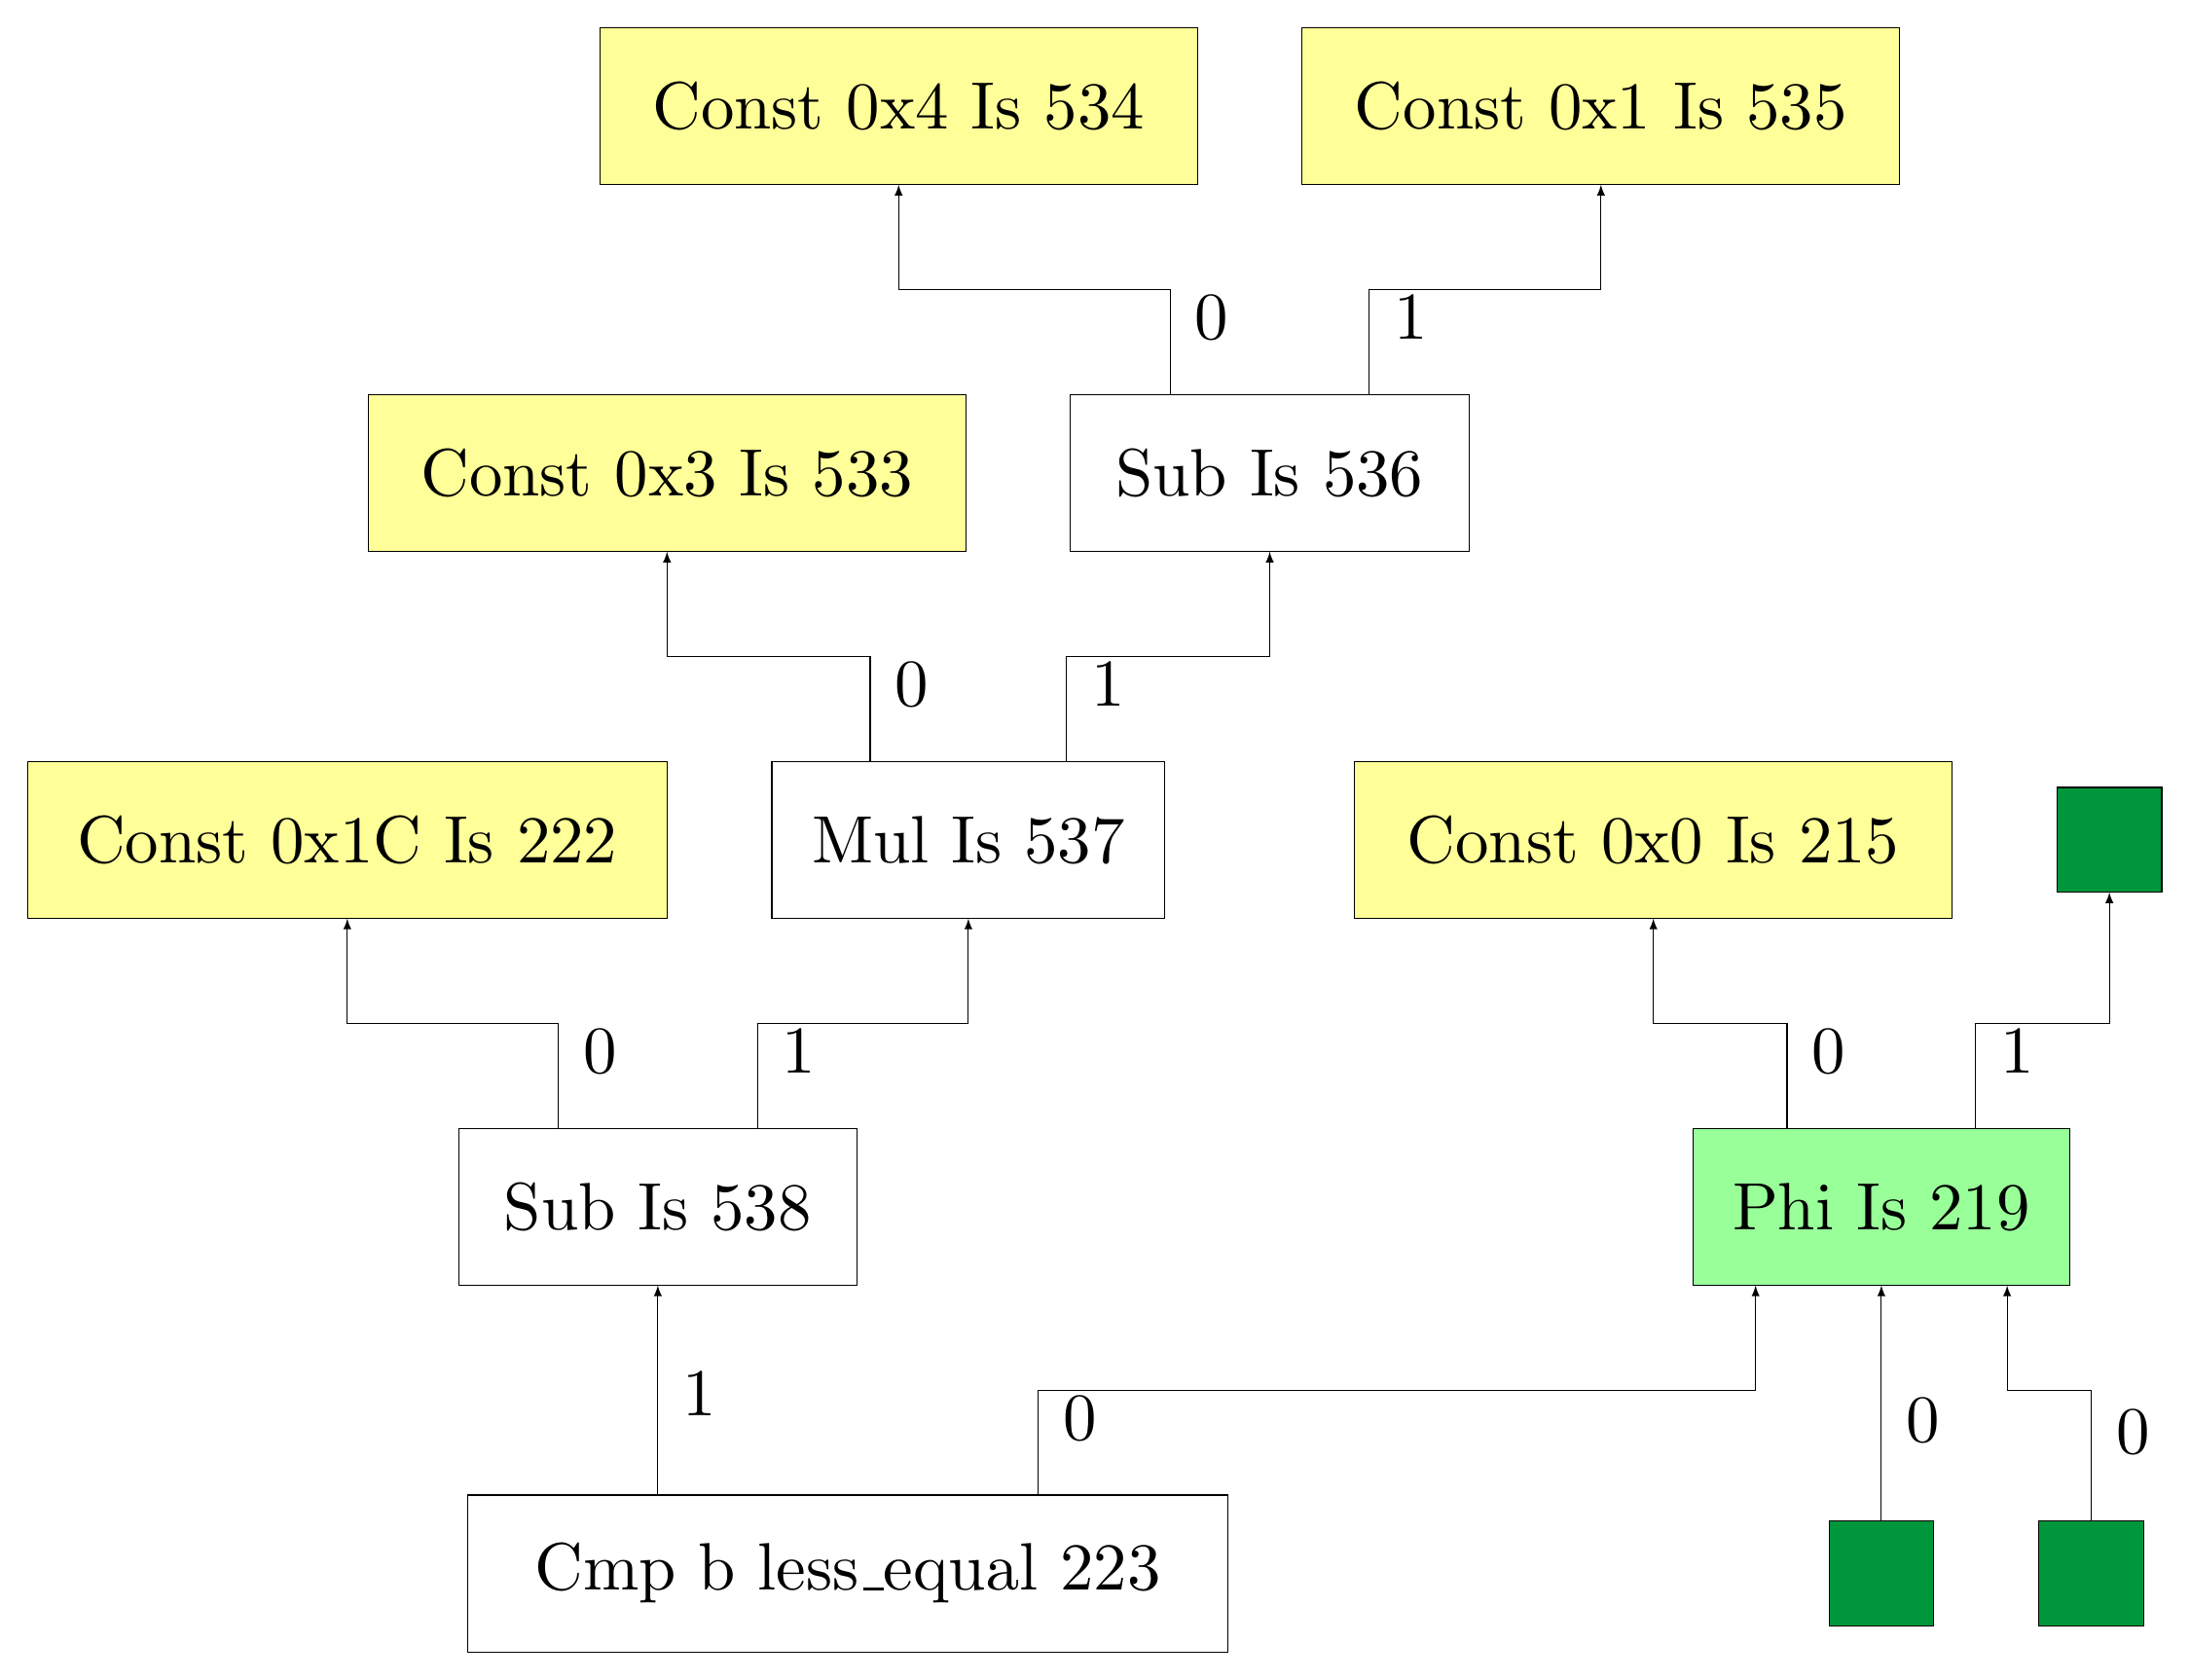
\begin{tikzpicture}
	\node[fill=color10, draw, minimum width=9.916129032258064cm, minimum height=2.0516129032258066cm] (n44) at (113.58092041890683cm ,-28.175483870967742cm) {};
	% 1 node layouts
	\node[scale=2.4868035190615836, transform shape] at (113.58092041890683cm ,-28.175483870967742cm) {Cmp b less\_equal 223};
	\node[fill=color11, draw, minimum width=4.9238709677419354cm, minimum height=2.0516129032258066cm] (n45) at (127.06635724686382cm ,-23.388387096774196cm) {};
	% 1 node layouts
	\node[scale=2.4868035190615836, transform shape] at (127.06635724686382cm ,-23.388387096774196cm) {Phi Is 219};
	\node[fill=color12, draw, minimum width=7.796129032258065cm, minimum height=2.0516129032258066cm] (n46) at (124.09151853718639cm ,-18.601290322580645cm) {};
	% 1 node layouts
	\node[scale=2.4868035190615836, transform shape] at (124.09151853718639cm ,-18.601290322580645cm) {Const 0x0 Is 215};
	\node[fill=color10, draw, minimum width=5.1974193548387095cm, minimum height=2.0516129032258066cm] (n47) at (111.10188816084231cm ,-23.388387096774196cm) {};
	% 1 node layouts
	\node[scale=2.4868035190615836, transform shape] at (111.10188816084231cm ,-23.388387096774196cm) {Sub Is 538};
	\node[fill=color12, draw, minimum width=8.343225806451613cm, minimum height=2.0516129032258066cm] (n48) at (107.04995267697134cm ,-18.601290322580645cm) {};
	% 1 node layouts
	\node[scale=2.4868035190615836, transform shape] at (107.04995267697134cm ,-18.601290322580645cm) {Const 0x1C Is 222};
	\node[fill=color10, draw, minimum width=5.129032258064516cm, minimum height=2.0516129032258066cm] (n49) at (115.15382364471328cm ,-18.601290322580645cm) {};
	% 1 node layouts
	\node[scale=2.4868035190615836, transform shape] at (115.15382364471328cm ,-18.601290322580645cm) {Mul Is 537};
	\node[fill=color12, draw, minimum width=7.796129032258065cm, minimum height=2.0516129032258066cm] (n50) at (111.22156558019715cm ,-13.814193548387097cm) {};
	% 1 node layouts
	\node[scale=2.4868035190615836, transform shape] at (111.22156558019715cm ,-13.814193548387097cm) {Const 0x3 Is 533};
	\node[fill=color10, draw, minimum width=5.1974193548387095cm, minimum height=2.0516129032258066cm] (n51) at (119.0860817092294cm ,-13.814193548387097cm) {};
	% 1 node layouts
	\node[scale=2.4868035190615836, transform shape] at (119.0860817092294cm ,-13.814193548387097cm) {Sub Is 536};
	\node[fill=color12, draw, minimum width=7.796129032258065cm, minimum height=2.0516129032258066cm] (n52) at (114.24377660170252cm ,-9.027096774193549cm) {};
	% 1 node layouts
	\node[scale=2.4868035190615836, transform shape] at (114.24377660170252cm ,-9.027096774193549cm) {Const 0x4 Is 534};
	\node[fill=color12, draw, minimum width=7.796129032258065cm, minimum height=2.0516129032258066cm] (n53) at (123.40764756944445cm ,-9.027096774193549cm) {};
	% 1 node layouts
	\node[scale=2.4868035190615836, transform shape] at (123.40764756944445cm ,-9.027096774193549cm) {Const 0x1 Is 535};
	\node[fill=color13, draw, minimum width=1.367741935483871cm, minimum height=1.367741935483871cm] (n54) at (129.80184111783154cm ,-28.175483870967742cm) {};
	\node[fill=color13, draw, minimum width=1.367741935483871cm, minimum height=1.367741935483871cm] (n55) at (130.04119595654123cm ,-18.601290322580645cm) {};
	\node[fill=color13, draw, minimum width=1.367741935483871cm, minimum height=1.367741935483871cm] (n56) at (127.06635724686382cm ,-28.175483870967742cm) {};
	\draw[color=color14, -latex] (116.05995267697135cm ,-27.14967741935484cm) -- (116.05995267697135cm ,-25.781935483870967cm) -- (125.42506692428317cm ,-25.781935483870967cm) -- (125.42506692428317cm ,-24.414193548387097cm);
	\node[] at (116.6070494511649cm ,-26.153790322580647cm) {
		\scalebox{2.4868035190615836}{0}
	};
	\draw[color=color14, -latex] (111.10188816084231cm ,-27.14967741935484cm) -- (111.10188816084231cm ,-24.414193548387097cm);
	\node[] at (111.64898493503586cm ,-25.837232862903228cm) {
		\scalebox{2.4868035190615836}{1}
	};
	\draw[color=color14, -latex] (125.83538950492833cm ,-22.36258064516129cm) -- (125.83538950492833cm ,-20.99483870967742cm) -- (124.09151853718639cm ,-20.99483870967742cm) -- (124.09151853718639cm ,-19.62709677419355cm);
	\node[] at (126.38248627912188cm ,-21.366693548387097cm) {
		\scalebox{2.4868035190615836}{0}
	};
	\draw[color=color14, -latex] (128.2973249887993cm ,-22.36258064516129cm) -- (128.2973249887993cm ,-20.99483870967742cm) -- (130.04119595654123cm ,-20.99483870967742cm) -- (130.04119595654123cm ,-19.28516129032258cm);
	\node[] at (128.84442176299285cm ,-21.366693548387097cm) {
		\scalebox{2.4868035190615836}{1}
	};
	\draw[color=color14, -latex] (109.80253332213263cm ,-22.36258064516129cm) -- (109.80253332213263cm ,-20.99483870967742cm) -- (107.04995267697134cm ,-20.99483870967742cm) -- (107.04995267697134cm ,-19.62709677419355cm);
	\node[] at (110.34963009632618cm ,-21.366693548387097cm) {
		\scalebox{2.4868035190615836}{0}
	};
	\draw[color=color14, -latex] (112.40124299955198cm ,-22.36258064516129cm) -- (112.40124299955198cm ,-20.99483870967742cm) -- (115.15382364471328cm ,-20.99483870967742cm) -- (115.15382364471328cm ,-19.62709677419355cm);
	\node[] at (112.94833977374553cm ,-21.366693548387097cm) {
		\scalebox{2.4868035190615836}{1}
	};
	\draw[color=color14, -latex] (113.87156558019714cm ,-17.575483870967744cm) -- (113.87156558019714cm ,-16.20774193548387cm) -- (111.22156558019715cm ,-16.20774193548387cm) -- (111.22156558019715cm ,-14.84cm);
	\node[] at (114.41866235439069cm ,-16.57959677419355cm) {
		\scalebox{2.4868035190615836}{0}
	};
	\draw[color=color14, -latex] (116.43608170922941cm ,-17.575483870967744cm) -- (116.43608170922941cm ,-16.20774193548387cm) -- (119.0860817092294cm ,-16.20774193548387cm) -- (119.0860817092294cm ,-14.84cm);
	\node[] at (116.98317848342296cm ,-16.57959677419355cm) {
		\scalebox{2.4868035190615836}{1}
	};
	\draw[color=color14, -latex] (117.78672687051973cm ,-12.788387096774194cm) -- (117.78672687051973cm ,-11.420645161290324cm) -- (114.24377660170252cm ,-11.420645161290324cm) -- (114.24377660170252cm ,-10.052903225806451cm);
	\node[] at (118.33382364471328cm ,-11.7925cm) {
		\scalebox{2.4868035190615836}{0}
	};
	\draw[color=color14, -latex] (120.38543654793908cm ,-12.788387096774194cm) -- (120.38543654793908cm ,-11.420645161290324cm) -- (123.40764756944445cm ,-11.420645161290324cm) -- (123.40764756944445cm ,-10.052903225806451cm);
	\node[] at (120.93253332213263cm ,-11.7925cm) {
		\scalebox{2.4868035190615836}{1}
	};
	\draw[color=color14, -latex] (129.80184111783154cm ,-27.491612903225807cm) -- (129.80184111783154cm ,-25.781935483870967cm) -- (128.70764756944445cm ,-25.781935483870967cm) -- (128.70764756944445cm ,-24.414193548387097cm);
	\node[] at (130.3489378920251cm ,-26.32475806451613cm) {
		\scalebox{2.4868035190615836}{0}
	};
	\draw[color=color14, -latex] (127.06635724686382cm ,-27.491612903225807cm) -- (127.06635724686382cm ,-24.414193548387097cm);
	\node[] at (127.61345402105736cm ,-26.179168346774194cm) {
		\scalebox{2.4868035190615836}{0}
	};
\end{tikzpicture}

    \caption{The changed header condition for \cref{fig:impl:fixup:duff:fixup-firm-loop} after constant folding}
    \label{fig:impl:fixup:header-cond:firm}
\end{figure}